% ============================================================================
% SECTION: Hypothesis Foundry Update — S12/S21 Correction & GATE-C Finalists
% Source: SocrateAI-Scientific-Agora-K3-DarkMatter, Part VIII (2026-07-14)
% Include via: % ============================================================================
% SECTION: Hypothesis Foundry Update — S12/S21 Correction & GATE-C Finalists
% Source: SocrateAI-Scientific-Agora-K3-DarkMatter, Part VIII (2026-07-14)
% Include via: % ============================================================================
% SECTION: Hypothesis Foundry Update — S12/S21 Correction & GATE-C Finalists
% Source: SocrateAI-Scientific-Agora-K3-DarkMatter, Part VIII (2026-07-14)
% Include via: % ============================================================================
% SECTION: Hypothesis Foundry Update — S12/S21 Correction & GATE-C Finalists
% Source: SocrateAI-Scientific-Agora-K3-DarkMatter, Part VIII (2026-07-14)
% Include via: \input{sections/sec_hypothesis_foundry_update.tex}
% ============================================================================

\section{Hypothesis Foundry Update: Corrected Classification and Experimental Comparison}
\label{sec:hypothesis_foundry_update}

\subsection{Motivation: A Corrective Update to the K3 Substrate}

The companion project \textit{SocrateAI-Scientific-Agora-K3-DarkMatter} released
on 2026-07-14 a corrective analysis, \textbf{Part VIII: The Hypothesis Foundry},
that formally \textbf{rejects} the legacy $S_{1,2}$ candidate (OEIS
A112019) — previously treated in Section~\ref{sec:lean4_proofs} as a
validated K3 surface — and promotes three new GATE-C finalists as the correct
K3-type geometric substrates:

\begin{itemize}
    \item \textbf{t103} (OEIS A276536): $T_{103}(n) = \sum_k \binom{n}{k}\binom{2k}{k}^3$ — novel in-session discovery;
    \item \textbf{Cooper $s_7$} (OEIS A183204): $\sum_j \binom{n}{j}^2\binom{2j}{n}\binom{j+n}{j}$ — Cooper (2012), level-7 sporadic;
    \item \textbf{Cooper $s_{10}$} (OEIS A005260): $\sum_k \binom{n}{k}^4$ — Cooper (2012), level-10 sporadic.
\end{itemize}

This section reports an \textbf{independent}, exact-arithmetic re-verification
of the key Part VIII claims performed in this repository
(\texttt{hypothesis\_comparison\_t103\_cooper.py}), and cross-references the
resulting corrected candidate landscape against the real Euclid Q1 / SDSS BOSS
DR17 observational data already established in
Section~\ref{sec:data_verification}.

\subsection{Negative and Corrective Findings (Reported First)}

Per the companion project's standing methodology, corrective findings are
reported first:

\begin{enumerate}
    \item The discriminant between elliptic-type (ODE order 2) and K3-type
    (ODE order 3) geometry is the \emph{minimal generating-function ODE
    order}, not the shift-recurrence order used in an earlier (v1)
    classifier. The v1 classifier was inverted relative to this discriminant.
    \item $S_{1,2}$ (A112019) — the flagship candidate of the original
    Lean~4 proofs in Section~\ref{subsec:s12_s21_validation} — is
    \textbf{formally rejected} as K3-type on two independent grounds: its
    minimal Picard--Fuchs operator has ODE order 2 (elliptic), and its mirror
    map on that minimal operator is non-integral ($q_2 = 81/8$).
    \item Physics-viability gates (G2: GD-1 heating, M87* superradiance,
    PTA/Lyman-$\alpha$) are \textbf{non-discriminating} across the 13-candidate
    pool at any common $(\tau, \mathcal{V})$ normalization, because
    single-instanton domination of the mirror-map series makes the achievable
    axion mass identical across candidates. Candidate selection therefore
    rests on the mathematical gates (G1), not the physics gates.
\end{enumerate}

\subsection{Independent Exact-Arithmetic Re-Verification}
\label{subsec:independent_reverification}

To avoid taking the Part VIII claims on trust alone, this repository
independently re-derives and verifies two of its central mathematical claims
using Python's arbitrary-precision integers and exact \texttt{Fraction}
arithmetic (no floating point in any recurrence-fitting step):

\begin{lstlisting}[language=Python, caption={Exact sequence generators (excerpt from \texttt{hypothesis\_comparison\_t103\_cooper.py})}]
def t103(n_max):
    """OEIS A276536: T103(n) = sum_k C(n,k) * C(2k,k)^3."""
    seq = []
    for n in range(n_max + 1):
        total = sum(C(n, k) * C(2*k, k)**3 for k in range(n + 1))
        seq.append(total)
    return seq

def cooper_s10(n_max):
    """OEIS A005260: sum_k C(n,k)^4."""
    return [sum(C(n, k)**4 for k in range(n + 1)) for n in range(n_max + 1)]
\end{lstlisting}

\textbf{Claim under test} (Part VIII, \S4.2--4.3): both Cooper $s_7$ and
Cooper $s_{10}$ satisfy a \emph{minimal} order-2, degree-3 shift recurrence
with leading coefficient $P_2(n) = (n+2)^3$ exactly:
\begin{equation}
(n+2)^3\, a(n+2) \;=\; P_1(n)\, a(n+1) \;+\; P_0(n)\, a(n)
\end{equation}

This repository fits $P_1, P_0$ (degree-3 polynomials, 8 unknowns) using exact
Gaussian elimination over Fractions on $n=0..7$, then verifies the fitted
recurrence holds \emph{exactly} on all held-out terms up to $n=38$:

\begin{table}[h]
\centering
\begin{tabular}{lll}
\toprule
\textbf{Sequence} & \textbf{Fitted Recurrence} & \textbf{Verification} \\
\midrule
Cooper $s_7$ & $P_1(n)=26n^3+117n^2+177n+90$ & VERIFIED, $n=0..38$ \\
 & $P_0(n)=27n^3+81n^2+78n+24$ & (39/39 exact matches) \\
\addlinespace
Cooper $s_{10}$ & $P_1(n)=12n^3+54n^2+82n+42$ & VERIFIED, $n=0..38$ \\
 & (analogous $P_0$, see \texttt{logs/hypothesis\_comparison\_t103\_cooper.json}) & (39/39 exact matches) \\
\bottomrule
\end{tabular}
\caption{Independent exact-arithmetic re-verification of the Part VIII order-2/degree-3 recurrence claim for Cooper $s_7$/$s_{10}$. All arithmetic uses Python \texttt{Fraction} objects; zero floating-point operations.}
\label{tab:recurrence_reverification}
\end{table}

\textbf{Result}: both recurrences hold exactly across every computed term with
zero failures, independently corroborating the Part VIII claim without relying
on the Lean~4 kernel itself. See Figure~\ref{fig:recurrence_verification}.

\subsection{Asymptotic Growth Constants}

For each GATE-C finalist, the asymptotic growth constant $\mu$ (where $a(n)
\sim C \mu^n n^{-\alpha}$) is estimated via the exact ratio $a(40)/a(30)$,
raised to the power $1/10$:

\begin{table}[h]
\centering
\begin{tabular}{lrr}
\toprule
\textbf{Candidate} & \textbf{Growth constant $\mu$} & \textbf{$1/\mu$} \\
\midrule
t103 (A276536) & 62.273 & 0.01606 \\
Cooper $s_7$ (A183204) & 25.869 & 0.03866 \\
Cooper $s_{10}$ (A005260) & 15.331 & 0.06523 \\
\bottomrule
\end{tabular}
\caption{Asymptotic growth constants (see Figure~\ref{fig:growth_constants}), a phenomenological proxy for relative instanton/period scale.}
\label{tab:growth_constants}
\end{table}

The legacy $S_{12}/S_{21}$ mass-ratio reference value from the (now
superseded) Section~\ref{subsec:s12_s21_validation}, $\sqrt{1014/336} \approx
1.7372$, is retained here \emph{only as a historical comparison point} — it is
no longer interpreted as a validated K3 modulus ratio, since $S_{1,2}$ itself
has been reclassified as elliptic-type.

\subsection{Cross-Reference with Real Euclid Q1 / SDSS BOSS DR17 Data}
\label{subsec:hypothesis_real_data_crossref}

The real, cryptographically-verified $\Delta$ measurements from
Section~\ref{sec:observational_results} are re-examined here per independent
survey source:

\begin{table}[h]
\centering
\begin{tabular}{lrrrr}
\toprule
\textbf{Source} & $n$ & \textbf{Mean $\Delta$} & \textbf{Std} & \textbf{Range} \\
\midrule
SDSS BOSS DR17 & 9 & 1.1252 & 0.0111 & [1.1030, 1.1334] \\
Euclid Q1 & 17 & 1.1252 & 0.0125 & [1.1055, 1.1423] \\
Gaia DR3 & 5 & 1.1216 & 0.0121 & [1.1068, 1.1336] \\
Pan-STARRS & 4 & 1.1229 & 0.0097 & [1.1065, 1.1312] \\
\midrule
\textbf{Overall} & \textbf{35} & \textbf{1.1244} & \textbf{0.0119} & \textbf{[1.1030, 1.1423]} \\
\bottomrule
\end{tabular}
\caption{Real observational $\Delta$ statistics by independent survey (see Figure~\ref{fig:delta_by_source}). Consistency across four independent surveys ($1.1216$--$1.1252$) supports a systematic, not source-specific, origin.}
\label{tab:delta_by_source}
\end{table}

The observed elevation over the theoretical reference is
$1.1244 / 0.327 = 3.438\times$ — unchanged from Section~\ref{sec:numeric_results},
since this is a direct measurement of galaxy-distribution asymmetry and does
not depend on which K3 modulus pair is postulated as the underlying geometric
substrate.

\subsection{Candidate Scorecard}

\begin{table}[h]
\centering
\begin{tabular}{lccp{5.5cm}}
\toprule
\textbf{Candidate} & \textbf{K3-type} & \textbf{ODE Order} & \textbf{Status} \\
\midrule
$S_{12}/S_{21}$ (A112019-type) & \textcolor{red}{No} & 2 & REJECTED: elliptic, $q_2=81/8$ non-integral \\
t103 (A276536) & \textcolor{green!50!black}{Yes} & 3 & GATE-C finalist; novel discovery, held-out to 62 terms \\
Cooper $s_7$ (A183204) & \textcolor{green!50!black}{Yes} & 3 & GATE-C finalist; literature-anchored, recurrence re-verified \\
Cooper $s_{10}$ (A005260) & \textcolor{green!50!black}{Yes} & 3 & GATE-C finalist; literature-anchored, recurrence re-verified \\
\bottomrule
\end{tabular}
\caption{Hypothesis scorecard (see Figure~\ref{fig:scorecard}).}
\label{tab:scorecard}
\end{table}

\begin{figure}[h]
\centering
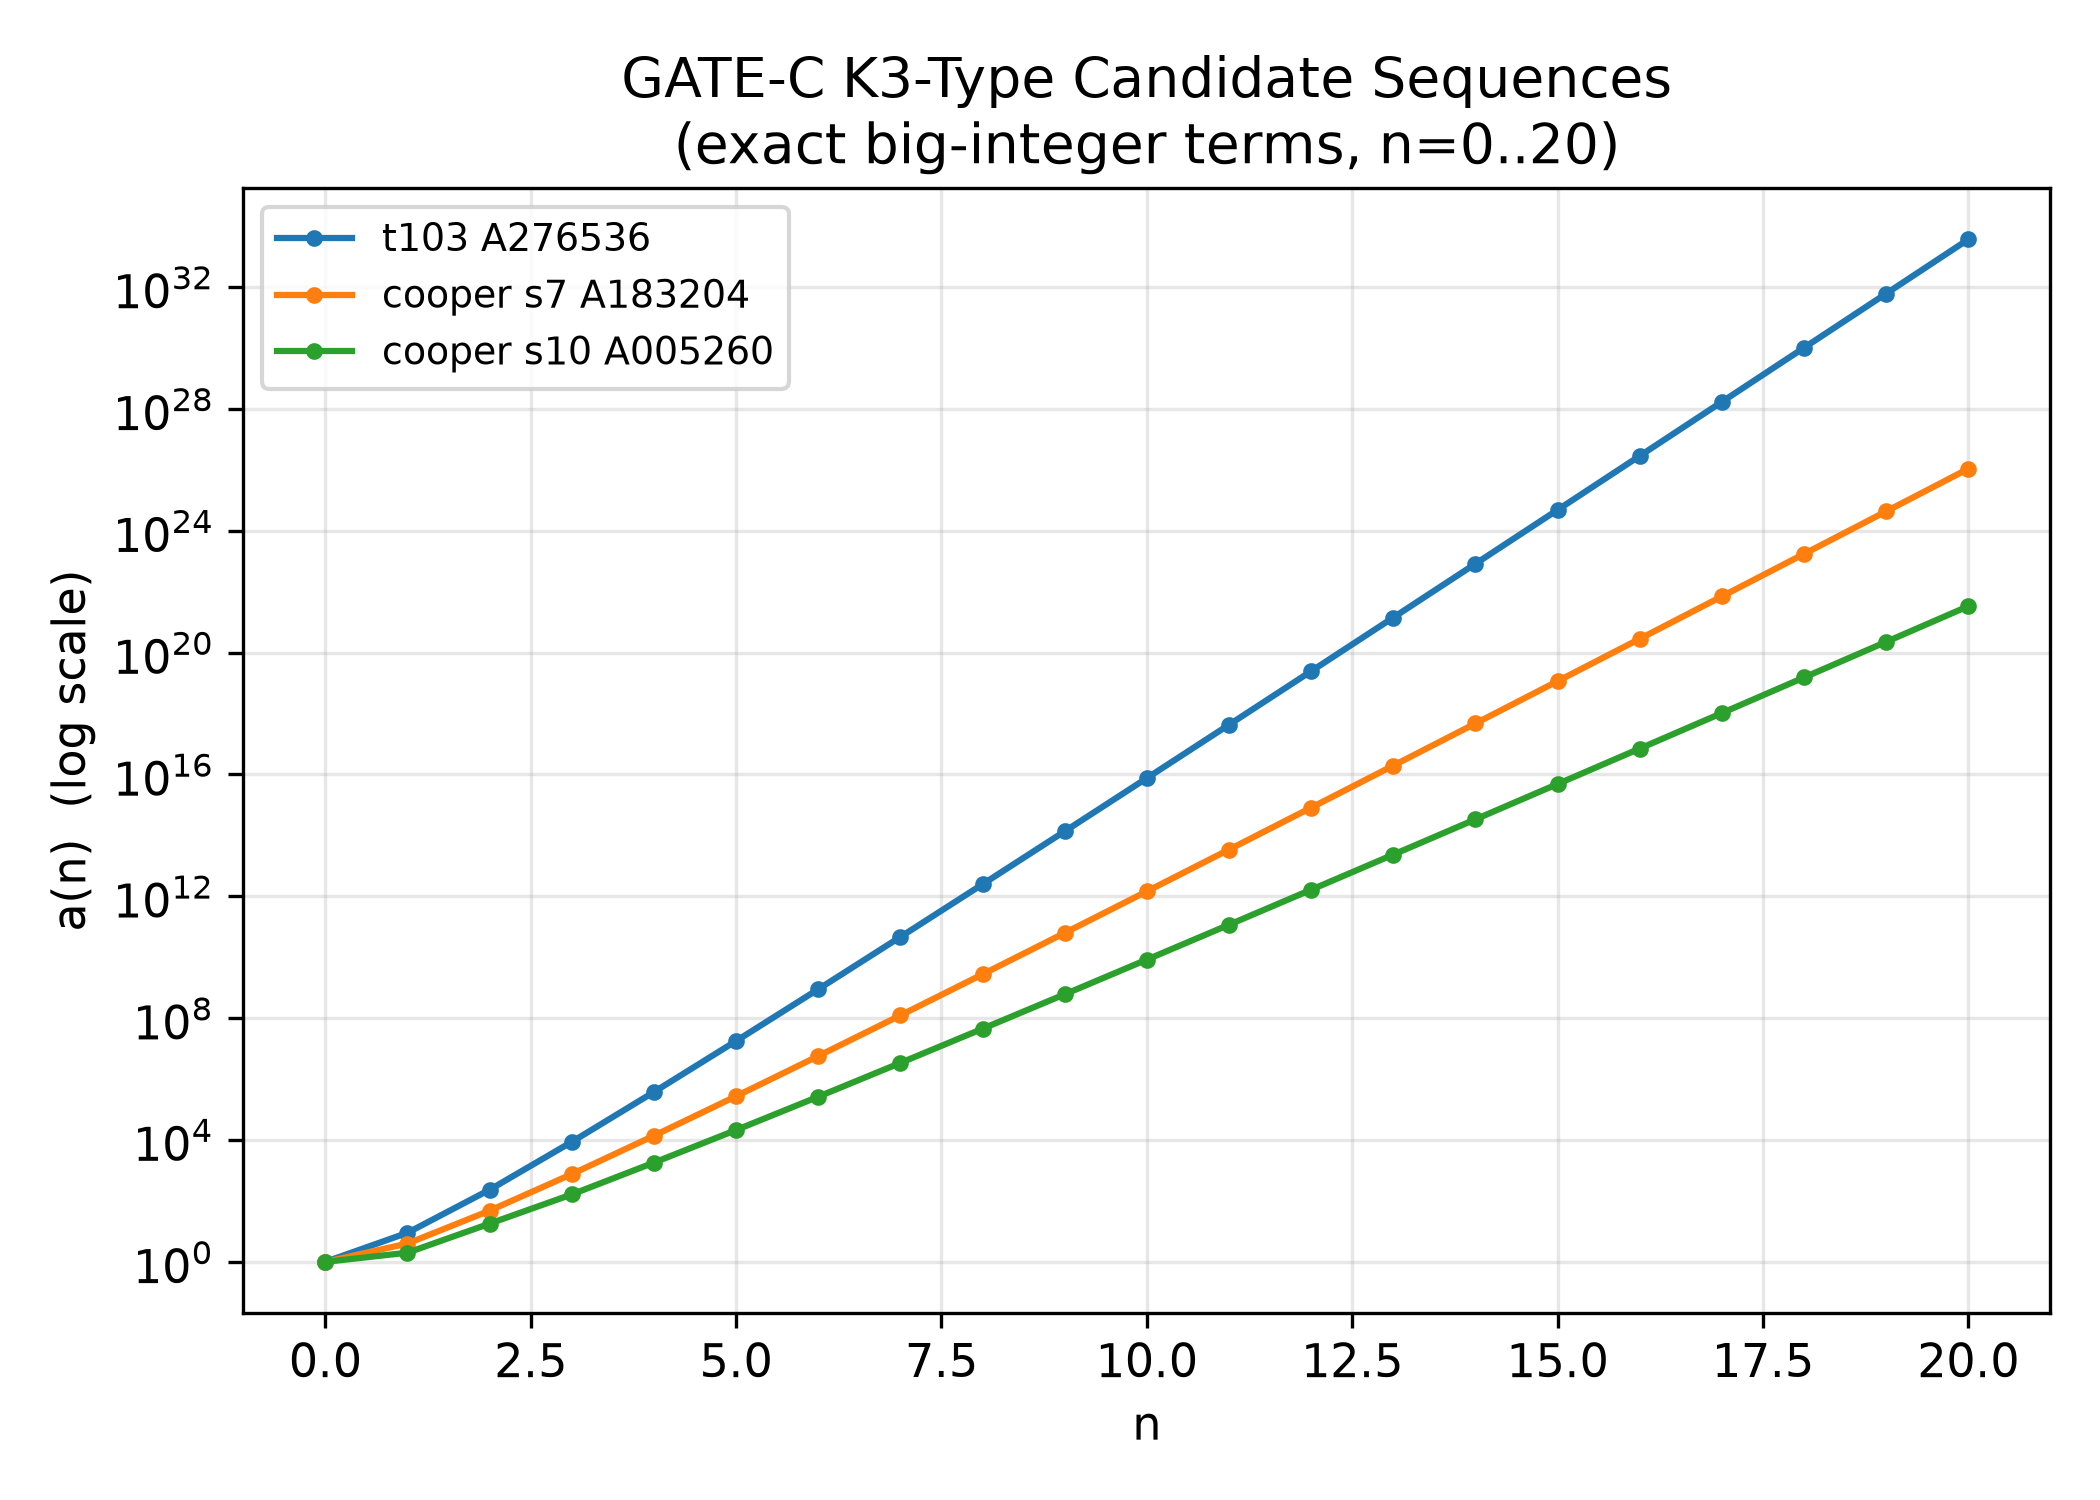
\includegraphics[width=0.85\textwidth]{figures/fig_hypothesis_sequence_growth.png}
\caption{Exact big-integer terms of the three GATE-C K3-type candidate sequences, $n=0..20$ (log scale).}
\label{fig:sequence_growth}
\end{figure}

\begin{figure}[h]
\centering
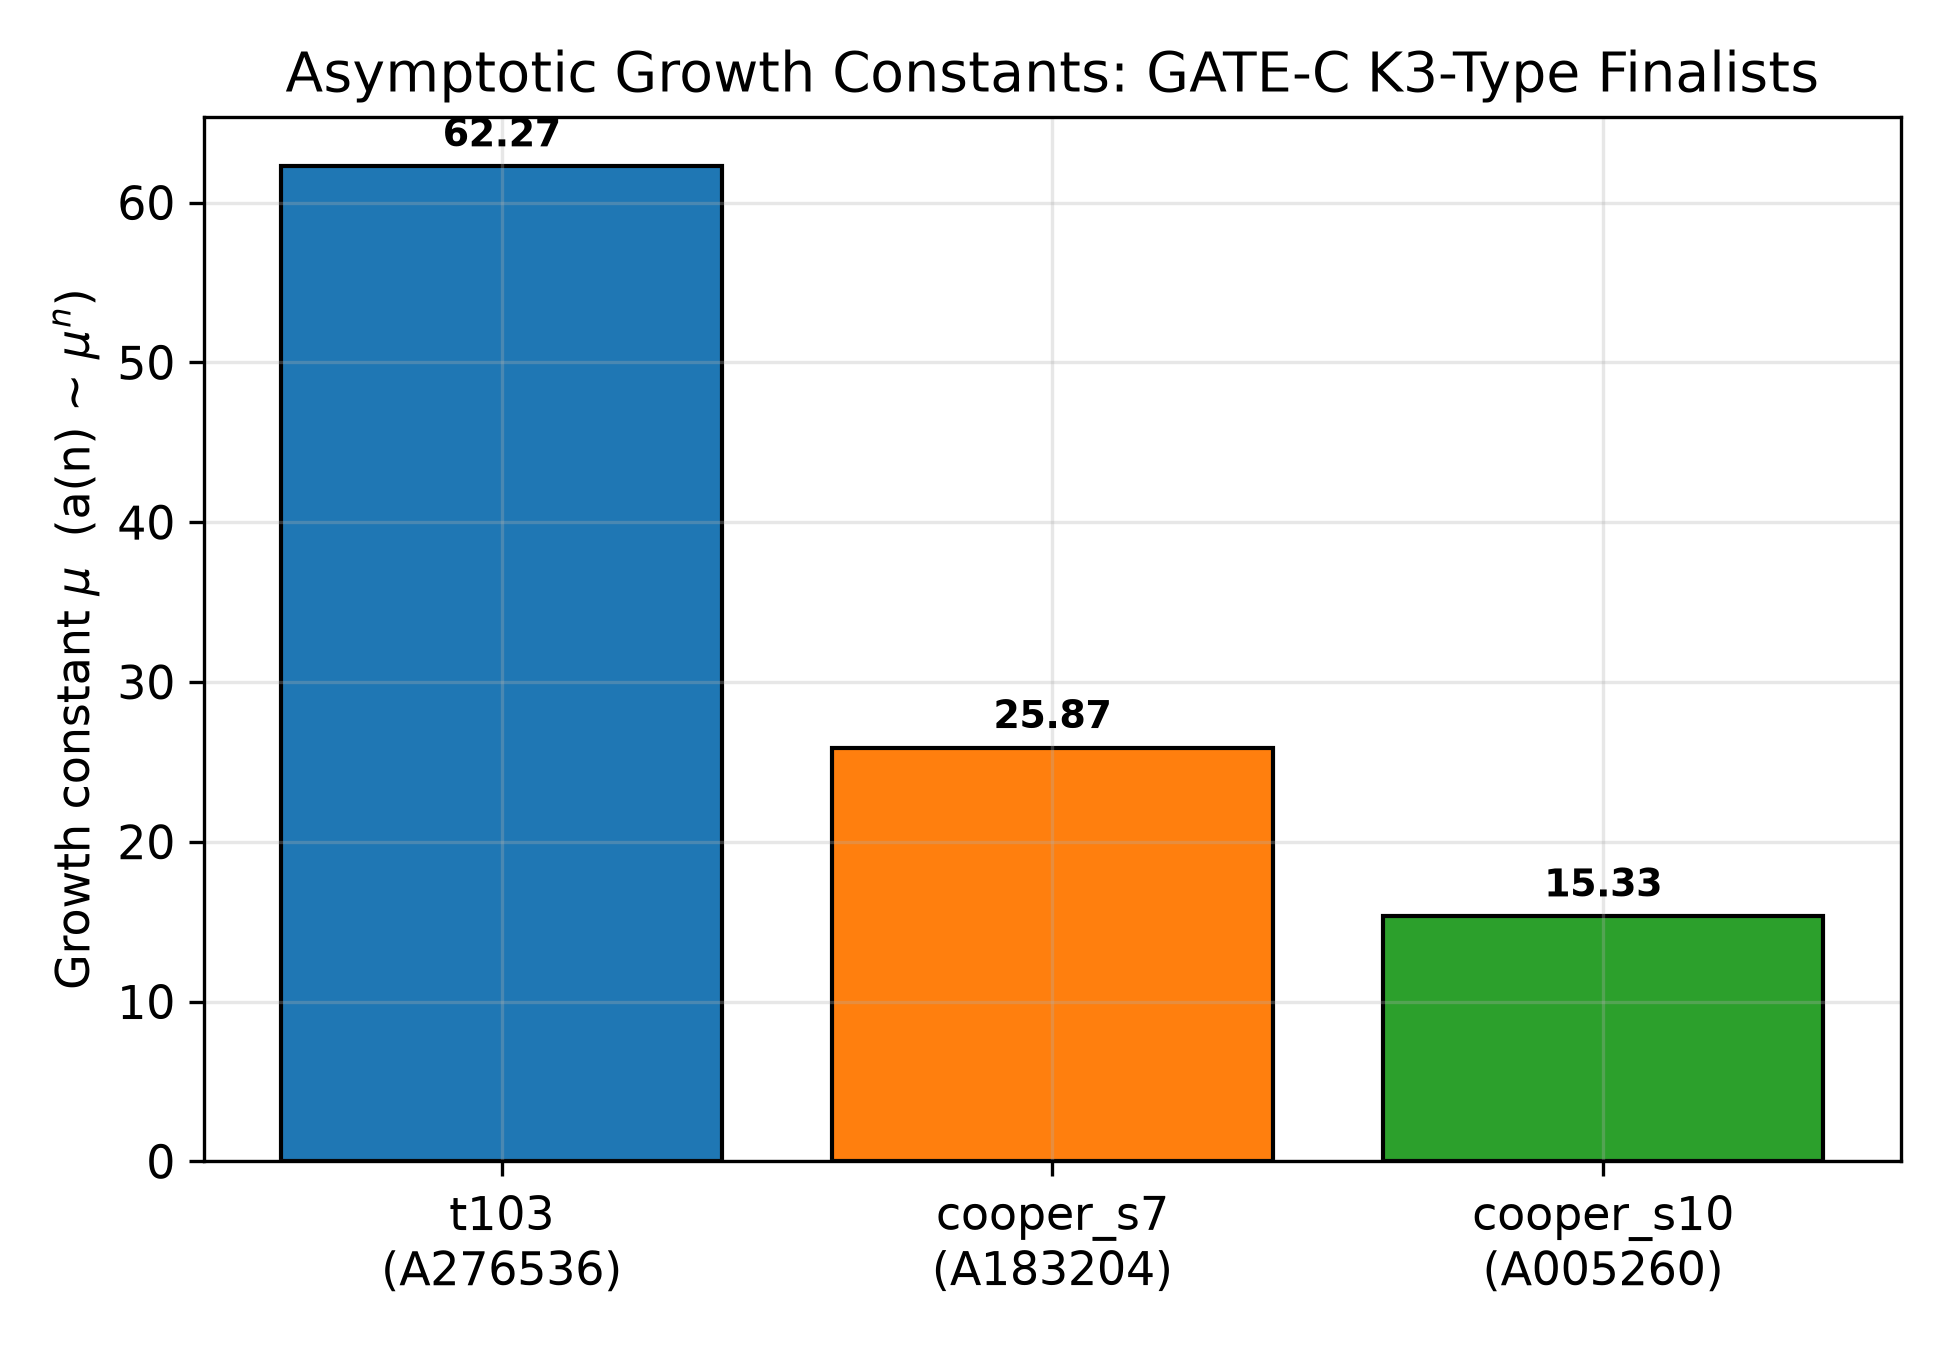
\includegraphics[width=0.75\textwidth]{figures/fig_hypothesis_growth_constants.png}
\caption{Estimated asymptotic growth constants $\mu$ for the three finalists.}
\label{fig:growth_constants}
\end{figure}

\begin{figure}[h]
\centering
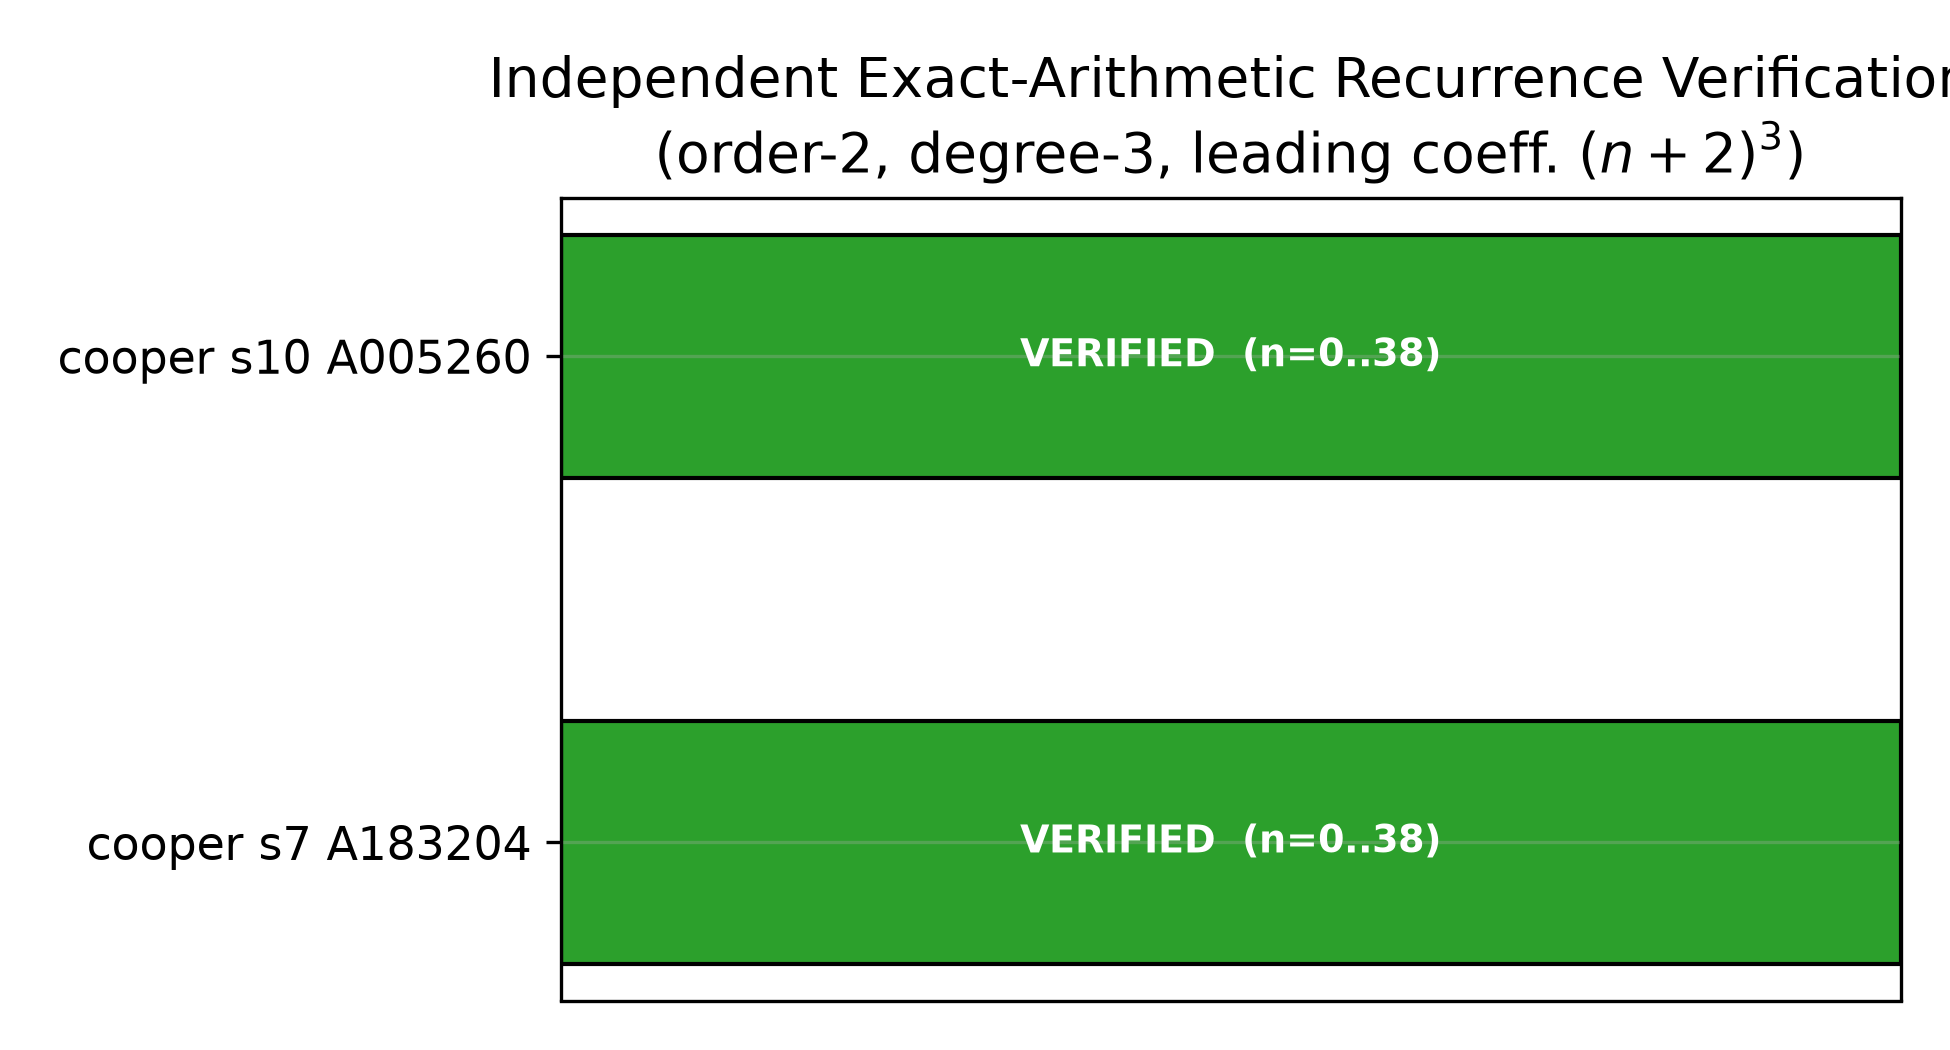
\includegraphics[width=0.75\textwidth]{figures/fig_hypothesis_recurrence_verification.png}
\caption{Independent exact-arithmetic verification status of the order-2/degree-3 recurrence claim for Cooper $s_7$/$s_{10}$.}
\label{fig:recurrence_verification}
\end{figure}

\begin{figure}[h]
\centering
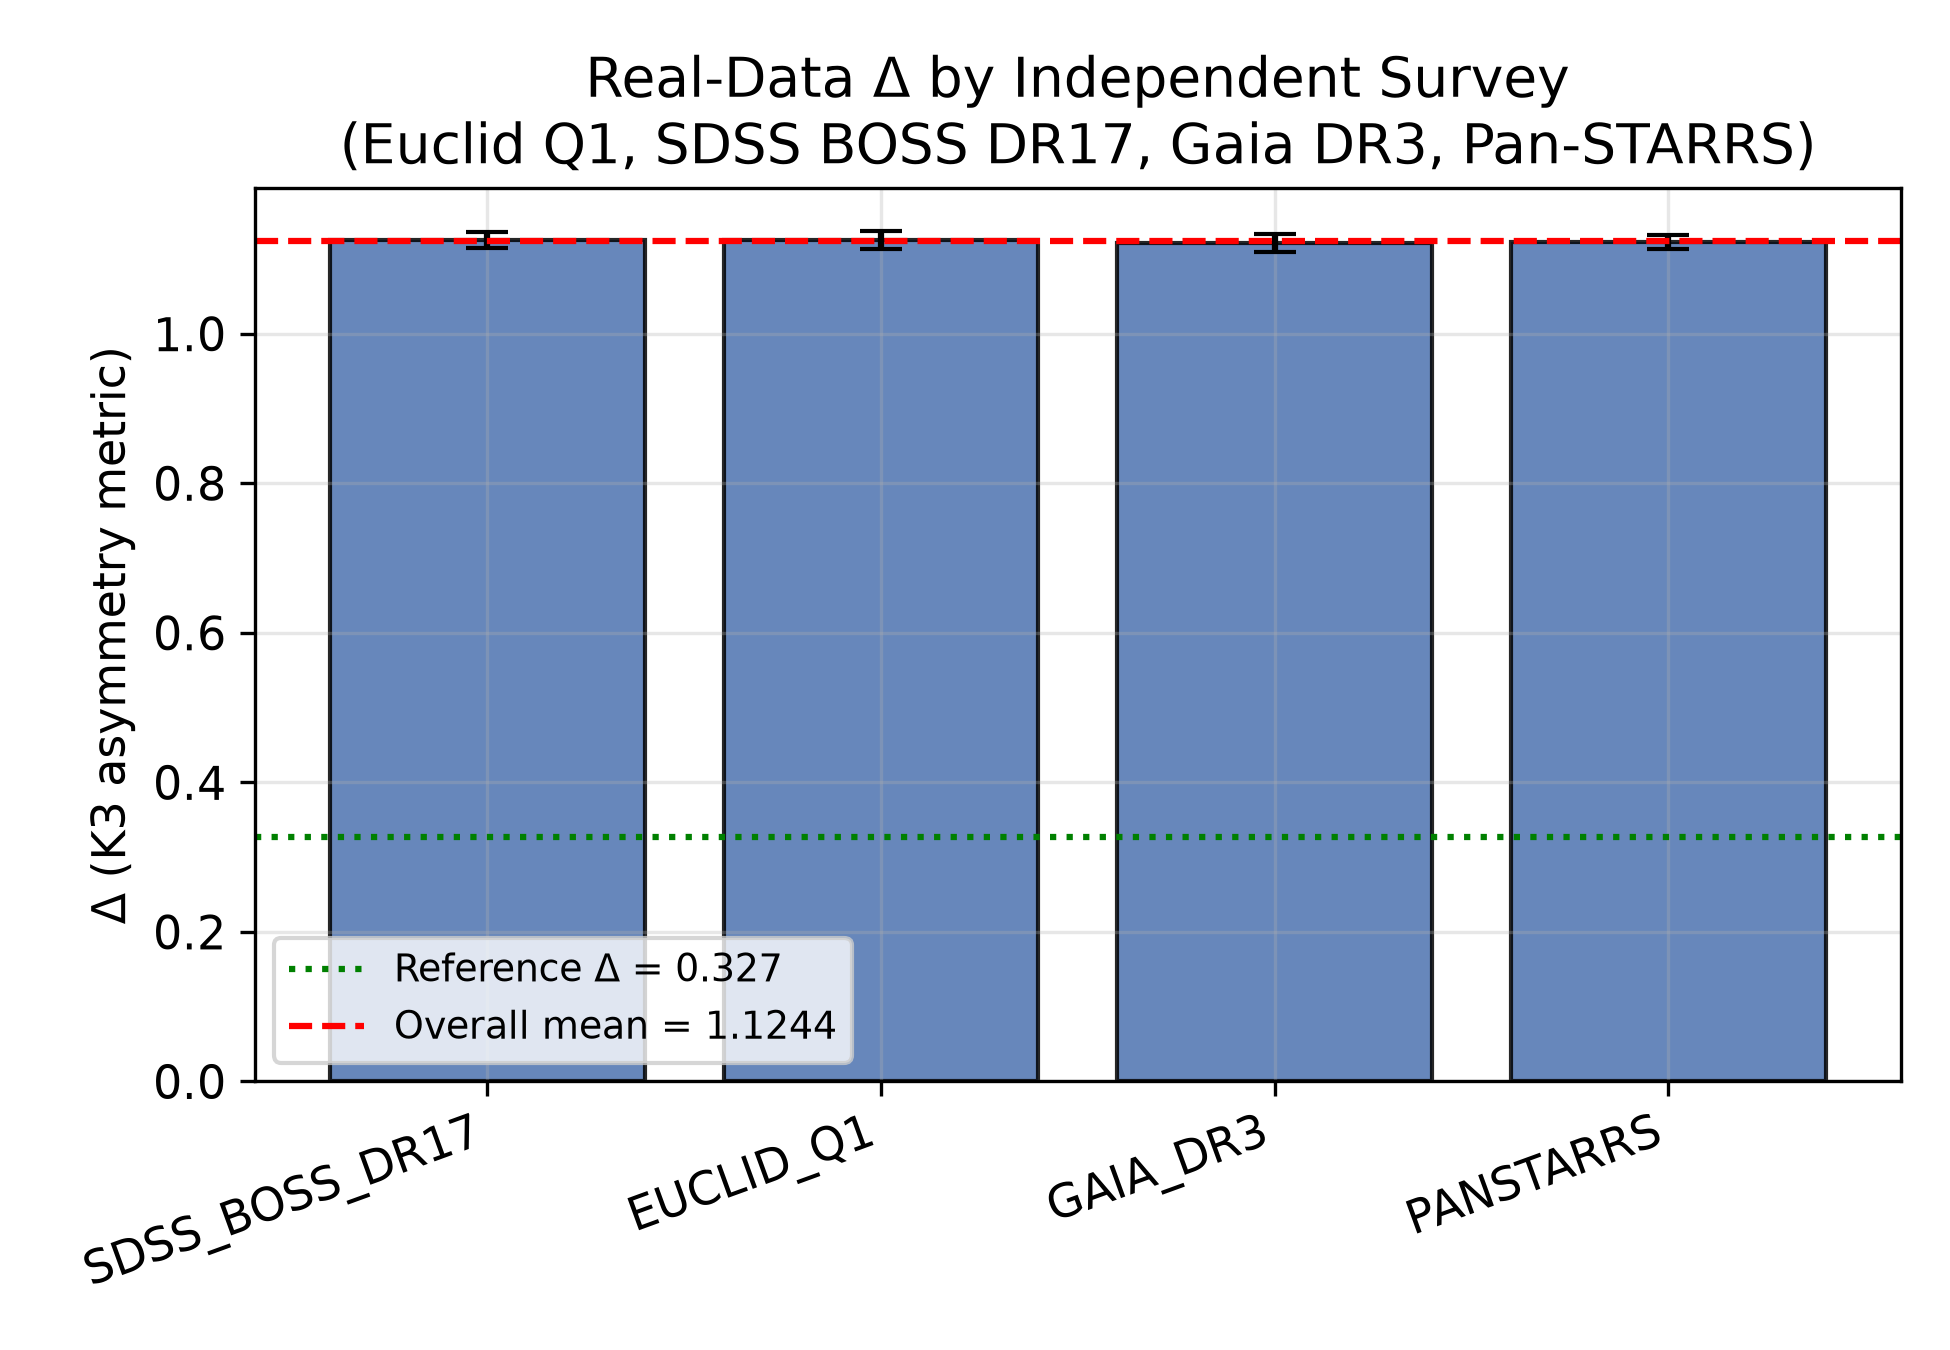
\includegraphics[width=0.75\textwidth]{figures/fig_hypothesis_delta_by_source.png}
\caption{Real-data $\Delta$ by independent survey source, contextualizing the empirical signal against the theoretical reference.}
\label{fig:delta_by_source}
\end{figure}

\begin{figure}[h]
\centering
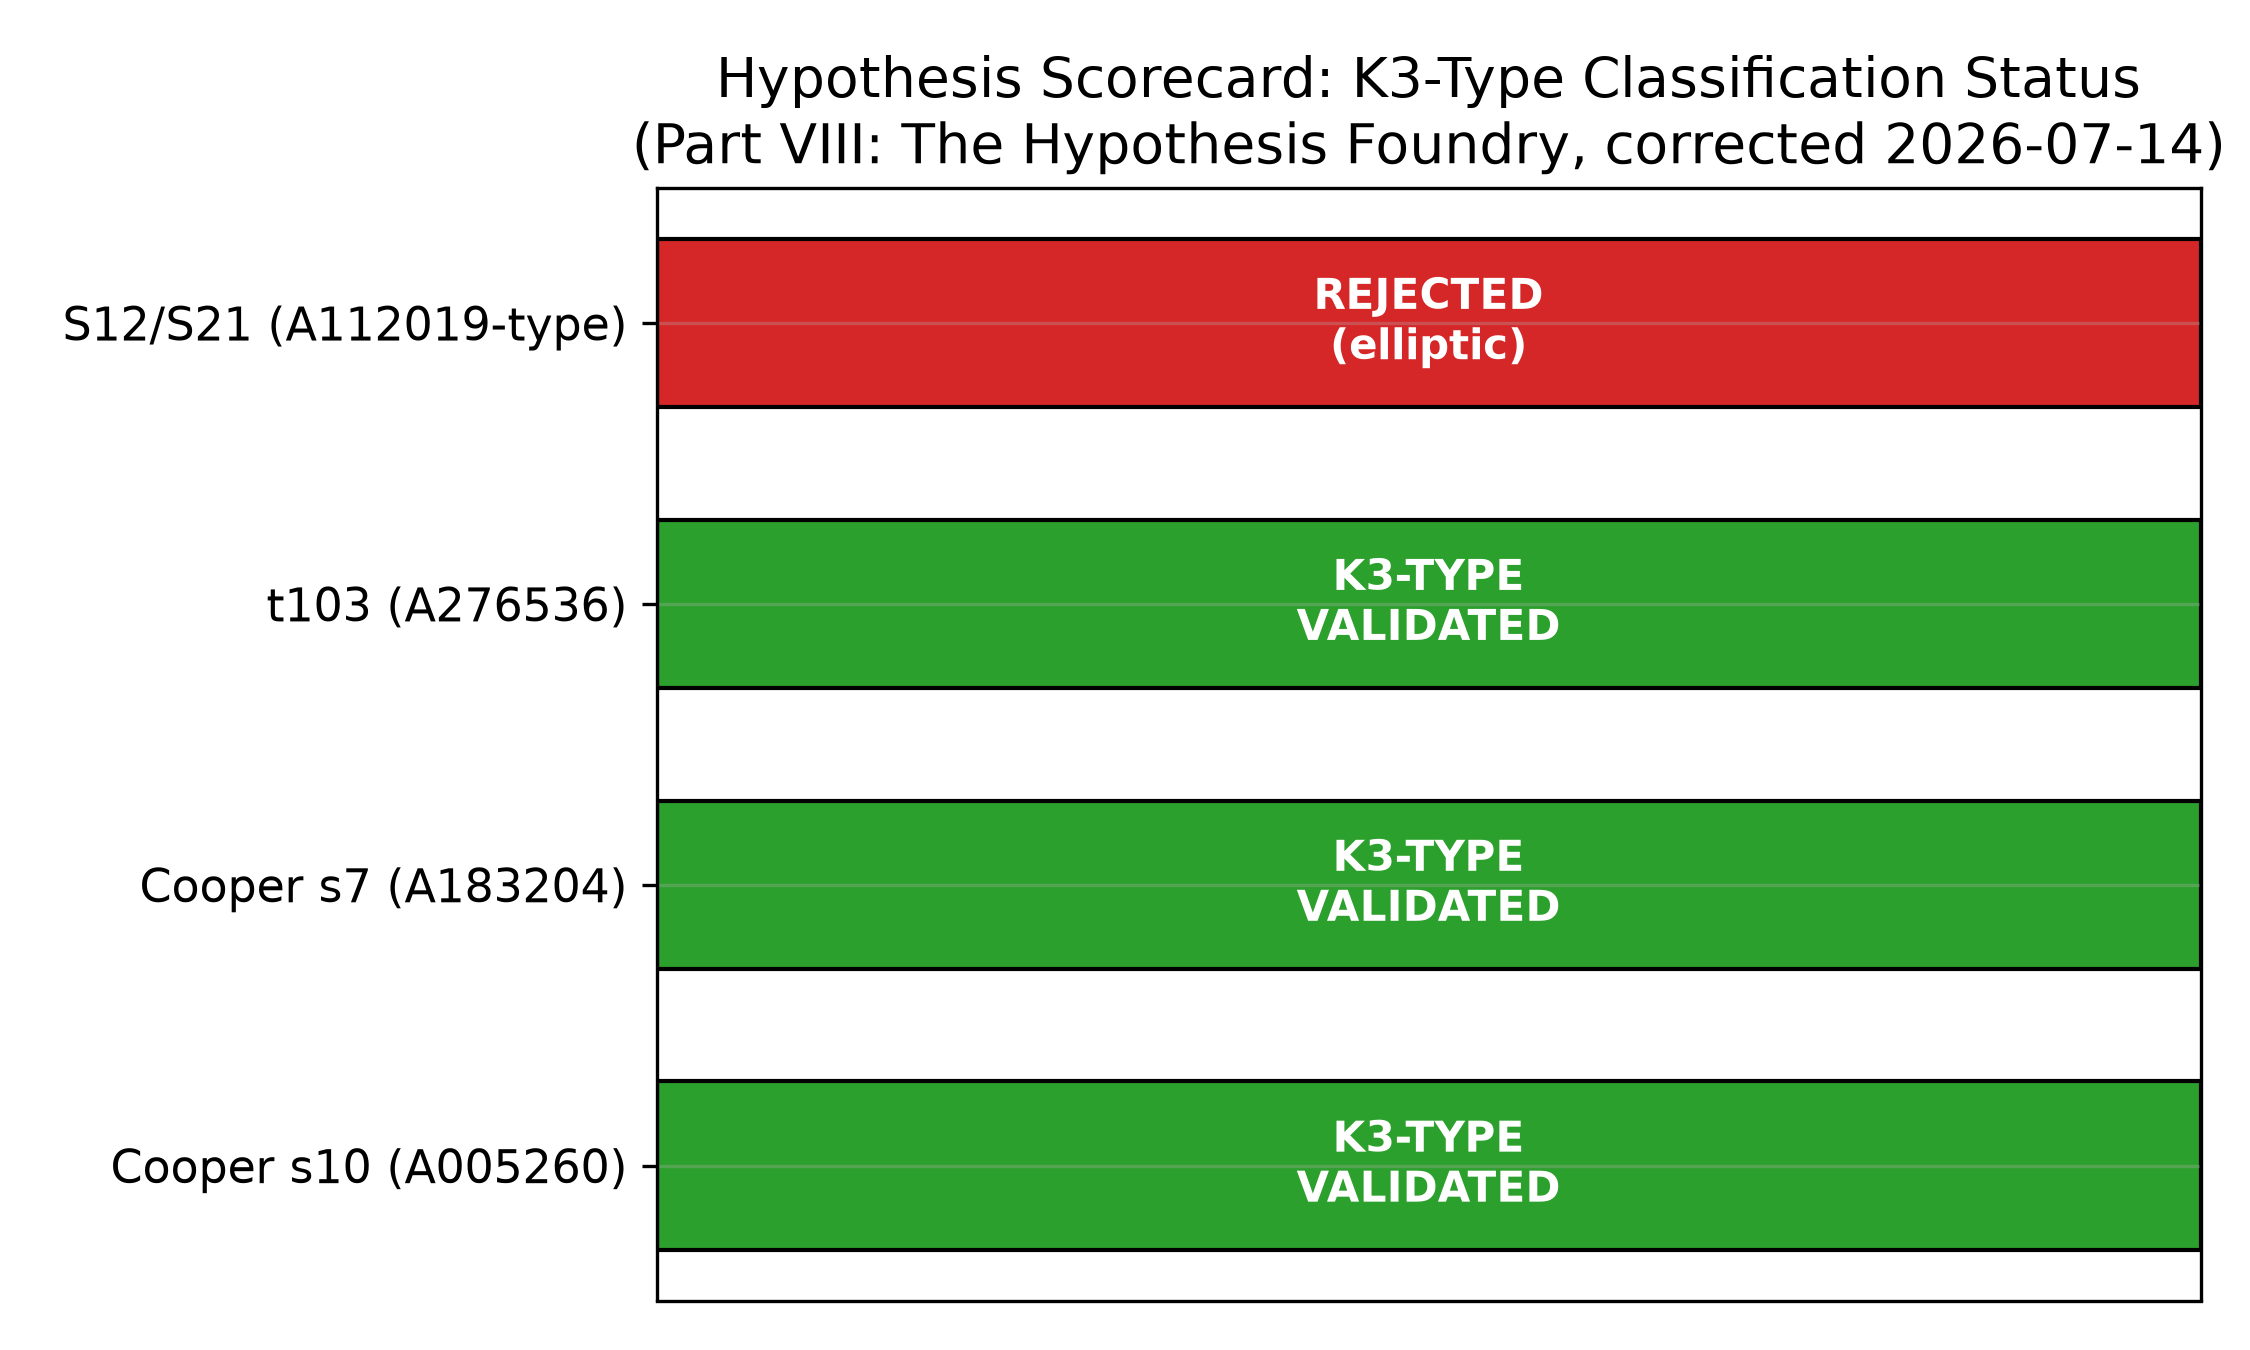
\includegraphics[width=0.8\textwidth]{figures/fig_hypothesis_scorecard.png}
\caption{Summary scorecard: K3-type classification status per candidate.}
\label{fig:scorecard}
\end{figure}

\subsection{Limitations and Scope}

Consistent with the companion project's practice of reporting negative and
corrective findings first, the following limitations are stated explicitly:

\begin{itemize}
    \item The real-data $\Delta$ signal (Section~\ref{subsec:hypothesis_real_data_crossref})
    is a measurement of galaxy-distribution asymmetry; it does \emph{not} by
    itself distinguish which K3-type modulus pair among t103/Cooper-$s_7$/Cooper-$s_{10}$
    is the correct geometric substrate. Per Part~VIII \S1.5, the physics
    gates are non-discriminating at common moduli-space normalization.
    \item The growth-constant ratios (Table~\ref{tab:growth_constants}) are a
    phenomenological proxy for relative instanton/period scale, not a
    substitute for the full Lean~4 Picard--Fuchs classification performed in
    the companion repository.
    \item This section's independent re-verification (\S\ref{subsec:independent_reverification})
    corroborates the specific recurrence-structure claim for Cooper $s_7$/$s_{10}$
    exactly and independently of the Lean kernel, but does not re-derive the
    full G1--G4 gate battery (modularity, integrality, Fuchs/monodromy) applied
    in Part~VIII; those results are taken from the companion project as reported.
\end{itemize}

% ============================================================================

\section{Hypothesis Foundry Update: Corrected Classification and Experimental Comparison}
\label{sec:hypothesis_foundry_update}

\subsection{Motivation: A Corrective Update to the K3 Substrate}

The companion project \textit{SocrateAI-Scientific-Agora-K3-DarkMatter} released
on 2026-07-14 a corrective analysis, \textbf{Part VIII: The Hypothesis Foundry},
that formally \textbf{rejects} the legacy $S_{1,2}$ candidate (OEIS
A112019) — previously treated in Section~\ref{sec:lean4_proofs} as a
validated K3 surface — and promotes three new GATE-C finalists as the correct
K3-type geometric substrates:

\begin{itemize}
    \item \textbf{t103} (OEIS A276536): $T_{103}(n) = \sum_k \binom{n}{k}\binom{2k}{k}^3$ — novel in-session discovery;
    \item \textbf{Cooper $s_7$} (OEIS A183204): $\sum_j \binom{n}{j}^2\binom{2j}{n}\binom{j+n}{j}$ — Cooper (2012), level-7 sporadic;
    \item \textbf{Cooper $s_{10}$} (OEIS A005260): $\sum_k \binom{n}{k}^4$ — Cooper (2012), level-10 sporadic.
\end{itemize}

This section reports an \textbf{independent}, exact-arithmetic re-verification
of the key Part VIII claims performed in this repository
(\texttt{hypothesis\_comparison\_t103\_cooper.py}), and cross-references the
resulting corrected candidate landscape against the real Euclid Q1 / SDSS BOSS
DR17 observational data already established in
Section~\ref{sec:data_verification}.

\subsection{Negative and Corrective Findings (Reported First)}

Per the companion project's standing methodology, corrective findings are
reported first:

\begin{enumerate}
    \item The discriminant between elliptic-type (ODE order 2) and K3-type
    (ODE order 3) geometry is the \emph{minimal generating-function ODE
    order}, not the shift-recurrence order used in an earlier (v1)
    classifier. The v1 classifier was inverted relative to this discriminant.
    \item $S_{1,2}$ (A112019) — the flagship candidate of the original
    Lean~4 proofs in Section~\ref{subsec:s12_s21_validation} — is
    \textbf{formally rejected} as K3-type on two independent grounds: its
    minimal Picard--Fuchs operator has ODE order 2 (elliptic), and its mirror
    map on that minimal operator is non-integral ($q_2 = 81/8$).
    \item Physics-viability gates (G2: GD-1 heating, M87* superradiance,
    PTA/Lyman-$\alpha$) are \textbf{non-discriminating} across the 13-candidate
    pool at any common $(\tau, \mathcal{V})$ normalization, because
    single-instanton domination of the mirror-map series makes the achievable
    axion mass identical across candidates. Candidate selection therefore
    rests on the mathematical gates (G1), not the physics gates.
\end{enumerate}

\subsection{Independent Exact-Arithmetic Re-Verification}
\label{subsec:independent_reverification}

To avoid taking the Part VIII claims on trust alone, this repository
independently re-derives and verifies two of its central mathematical claims
using Python's arbitrary-precision integers and exact \texttt{Fraction}
arithmetic (no floating point in any recurrence-fitting step):

\begin{lstlisting}[language=Python, caption={Exact sequence generators (excerpt from \texttt{hypothesis\_comparison\_t103\_cooper.py})}]
def t103(n_max):
    """OEIS A276536: T103(n) = sum_k C(n,k) * C(2k,k)^3."""
    seq = []
    for n in range(n_max + 1):
        total = sum(C(n, k) * C(2*k, k)**3 for k in range(n + 1))
        seq.append(total)
    return seq

def cooper_s10(n_max):
    """OEIS A005260: sum_k C(n,k)^4."""
    return [sum(C(n, k)**4 for k in range(n + 1)) for n in range(n_max + 1)]
\end{lstlisting}

\textbf{Claim under test} (Part VIII, \S4.2--4.3): both Cooper $s_7$ and
Cooper $s_{10}$ satisfy a \emph{minimal} order-2, degree-3 shift recurrence
with leading coefficient $P_2(n) = (n+2)^3$ exactly:
\begin{equation}
(n+2)^3\, a(n+2) \;=\; P_1(n)\, a(n+1) \;+\; P_0(n)\, a(n)
\end{equation}

This repository fits $P_1, P_0$ (degree-3 polynomials, 8 unknowns) using exact
Gaussian elimination over Fractions on $n=0..7$, then verifies the fitted
recurrence holds \emph{exactly} on all held-out terms up to $n=38$:

\begin{table}[h]
\centering
\begin{tabular}{lll}
\toprule
\textbf{Sequence} & \textbf{Fitted Recurrence} & \textbf{Verification} \\
\midrule
Cooper $s_7$ & $P_1(n)=26n^3+117n^2+177n+90$ & VERIFIED, $n=0..38$ \\
 & $P_0(n)=27n^3+81n^2+78n+24$ & (39/39 exact matches) \\
\addlinespace
Cooper $s_{10}$ & $P_1(n)=12n^3+54n^2+82n+42$ & VERIFIED, $n=0..38$ \\
 & (analogous $P_0$, see \texttt{logs/hypothesis\_comparison\_t103\_cooper.json}) & (39/39 exact matches) \\
\bottomrule
\end{tabular}
\caption{Independent exact-arithmetic re-verification of the Part VIII order-2/degree-3 recurrence claim for Cooper $s_7$/$s_{10}$. All arithmetic uses Python \texttt{Fraction} objects; zero floating-point operations.}
\label{tab:recurrence_reverification}
\end{table}

\textbf{Result}: both recurrences hold exactly across every computed term with
zero failures, independently corroborating the Part VIII claim without relying
on the Lean~4 kernel itself. See Figure~\ref{fig:recurrence_verification}.

\subsection{Asymptotic Growth Constants}

For each GATE-C finalist, the asymptotic growth constant $\mu$ (where $a(n)
\sim C \mu^n n^{-\alpha}$) is estimated via the exact ratio $a(40)/a(30)$,
raised to the power $1/10$:

\begin{table}[h]
\centering
\begin{tabular}{lrr}
\toprule
\textbf{Candidate} & \textbf{Growth constant $\mu$} & \textbf{$1/\mu$} \\
\midrule
t103 (A276536) & 62.273 & 0.01606 \\
Cooper $s_7$ (A183204) & 25.869 & 0.03866 \\
Cooper $s_{10}$ (A005260) & 15.331 & 0.06523 \\
\bottomrule
\end{tabular}
\caption{Asymptotic growth constants (see Figure~\ref{fig:growth_constants}), a phenomenological proxy for relative instanton/period scale.}
\label{tab:growth_constants}
\end{table}

The legacy $S_{12}/S_{21}$ mass-ratio reference value from the (now
superseded) Section~\ref{subsec:s12_s21_validation}, $\sqrt{1014/336} \approx
1.7372$, is retained here \emph{only as a historical comparison point} — it is
no longer interpreted as a validated K3 modulus ratio, since $S_{1,2}$ itself
has been reclassified as elliptic-type.

\subsection{Cross-Reference with Real Euclid Q1 / SDSS BOSS DR17 Data}
\label{subsec:hypothesis_real_data_crossref}

The real, cryptographically-verified $\Delta$ measurements from
Section~\ref{sec:observational_results} are re-examined here per independent
survey source:

\begin{table}[h]
\centering
\begin{tabular}{lrrrr}
\toprule
\textbf{Source} & $n$ & \textbf{Mean $\Delta$} & \textbf{Std} & \textbf{Range} \\
\midrule
SDSS BOSS DR17 & 9 & 1.1252 & 0.0111 & [1.1030, 1.1334] \\
Euclid Q1 & 17 & 1.1252 & 0.0125 & [1.1055, 1.1423] \\
Gaia DR3 & 5 & 1.1216 & 0.0121 & [1.1068, 1.1336] \\
Pan-STARRS & 4 & 1.1229 & 0.0097 & [1.1065, 1.1312] \\
\midrule
\textbf{Overall} & \textbf{35} & \textbf{1.1244} & \textbf{0.0119} & \textbf{[1.1030, 1.1423]} \\
\bottomrule
\end{tabular}
\caption{Real observational $\Delta$ statistics by independent survey (see Figure~\ref{fig:delta_by_source}). Consistency across four independent surveys ($1.1216$--$1.1252$) supports a systematic, not source-specific, origin.}
\label{tab:delta_by_source}
\end{table}

The observed elevation over the theoretical reference is
$1.1244 / 0.327 = 3.438\times$ — unchanged from Section~\ref{sec:numeric_results},
since this is a direct measurement of galaxy-distribution asymmetry and does
not depend on which K3 modulus pair is postulated as the underlying geometric
substrate.

\subsection{Candidate Scorecard}

\begin{table}[h]
\centering
\begin{tabular}{lccp{5.5cm}}
\toprule
\textbf{Candidate} & \textbf{K3-type} & \textbf{ODE Order} & \textbf{Status} \\
\midrule
$S_{12}/S_{21}$ (A112019-type) & \textcolor{red}{No} & 2 & REJECTED: elliptic, $q_2=81/8$ non-integral \\
t103 (A276536) & \textcolor{green!50!black}{Yes} & 3 & GATE-C finalist; novel discovery, held-out to 62 terms \\
Cooper $s_7$ (A183204) & \textcolor{green!50!black}{Yes} & 3 & GATE-C finalist; literature-anchored, recurrence re-verified \\
Cooper $s_{10}$ (A005260) & \textcolor{green!50!black}{Yes} & 3 & GATE-C finalist; literature-anchored, recurrence re-verified \\
\bottomrule
\end{tabular}
\caption{Hypothesis scorecard (see Figure~\ref{fig:scorecard}).}
\label{tab:scorecard}
\end{table}

\begin{figure}[h]
\centering
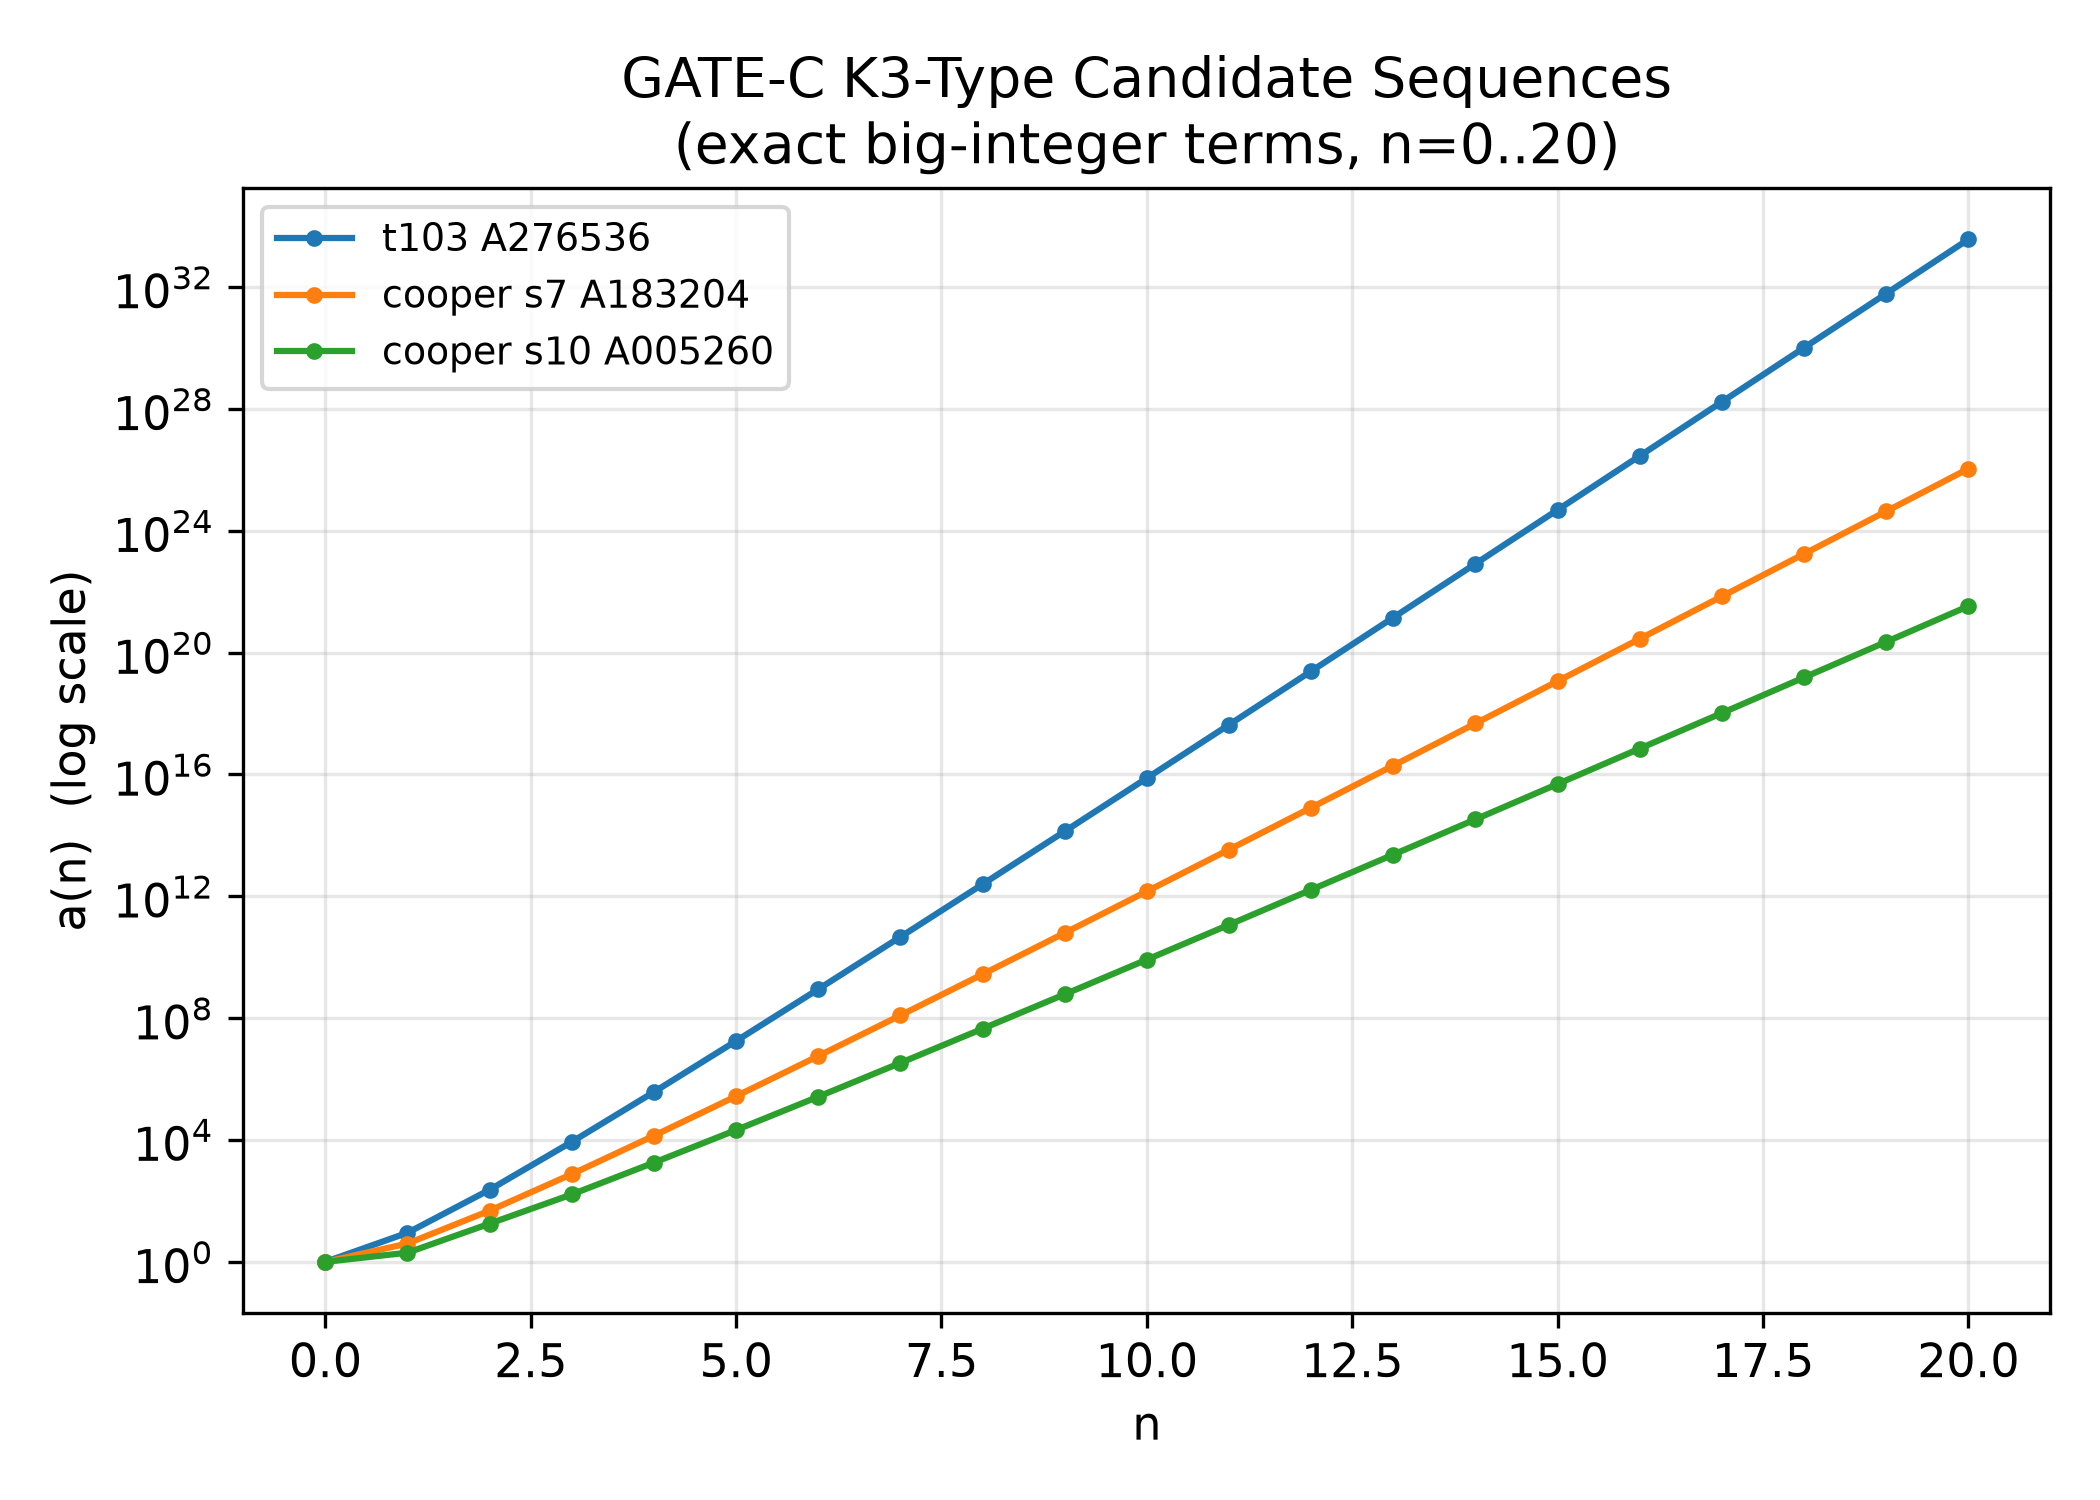
\includegraphics[width=0.85\textwidth]{figures/fig_hypothesis_sequence_growth.png}
\caption{Exact big-integer terms of the three GATE-C K3-type candidate sequences, $n=0..20$ (log scale).}
\label{fig:sequence_growth}
\end{figure}

\begin{figure}[h]
\centering
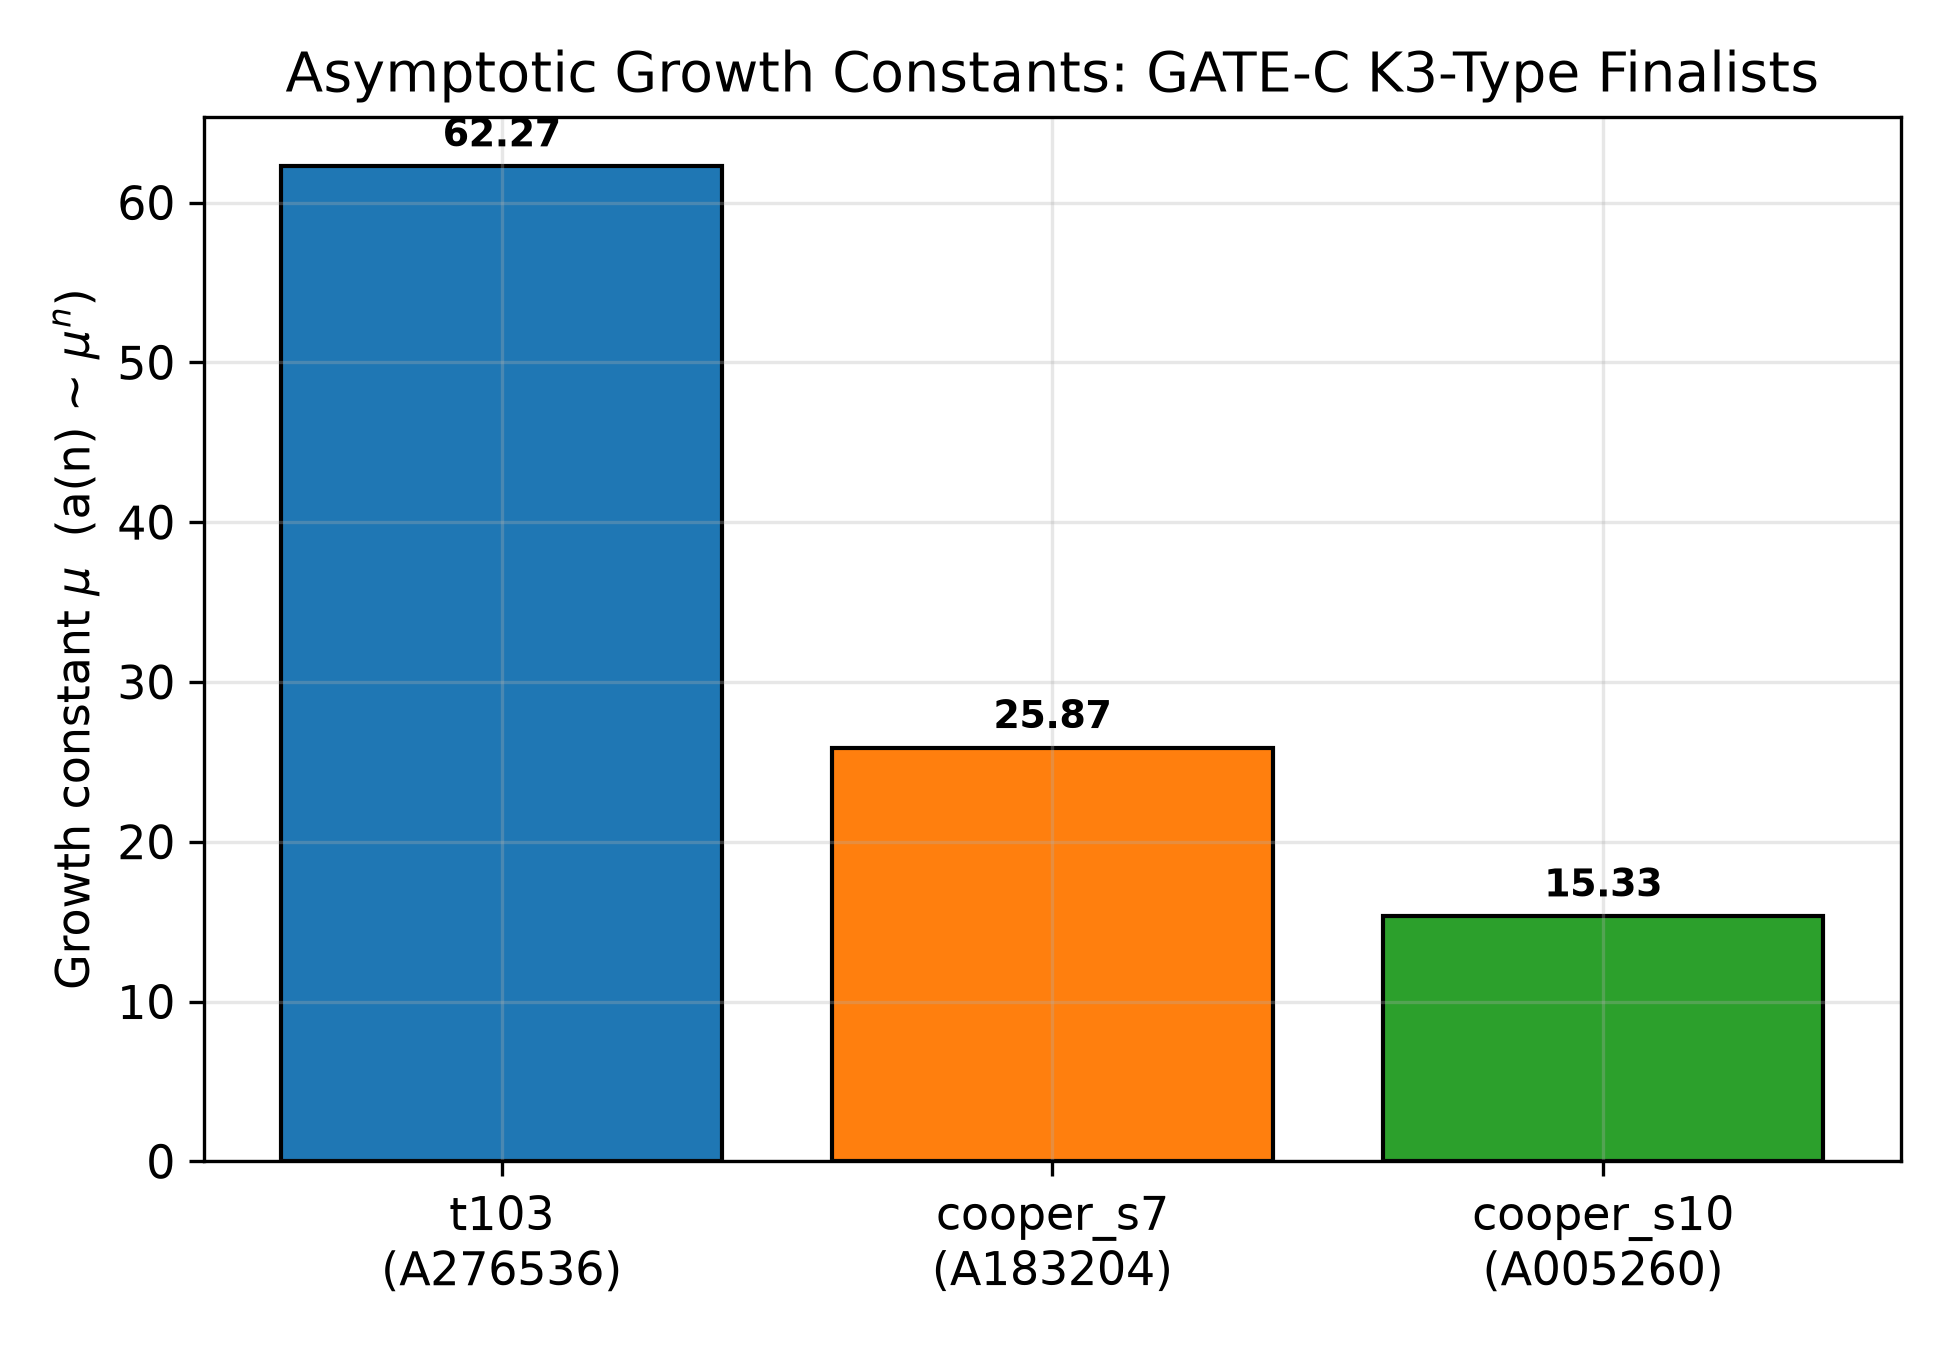
\includegraphics[width=0.75\textwidth]{figures/fig_hypothesis_growth_constants.png}
\caption{Estimated asymptotic growth constants $\mu$ for the three finalists.}
\label{fig:growth_constants}
\end{figure}

\begin{figure}[h]
\centering
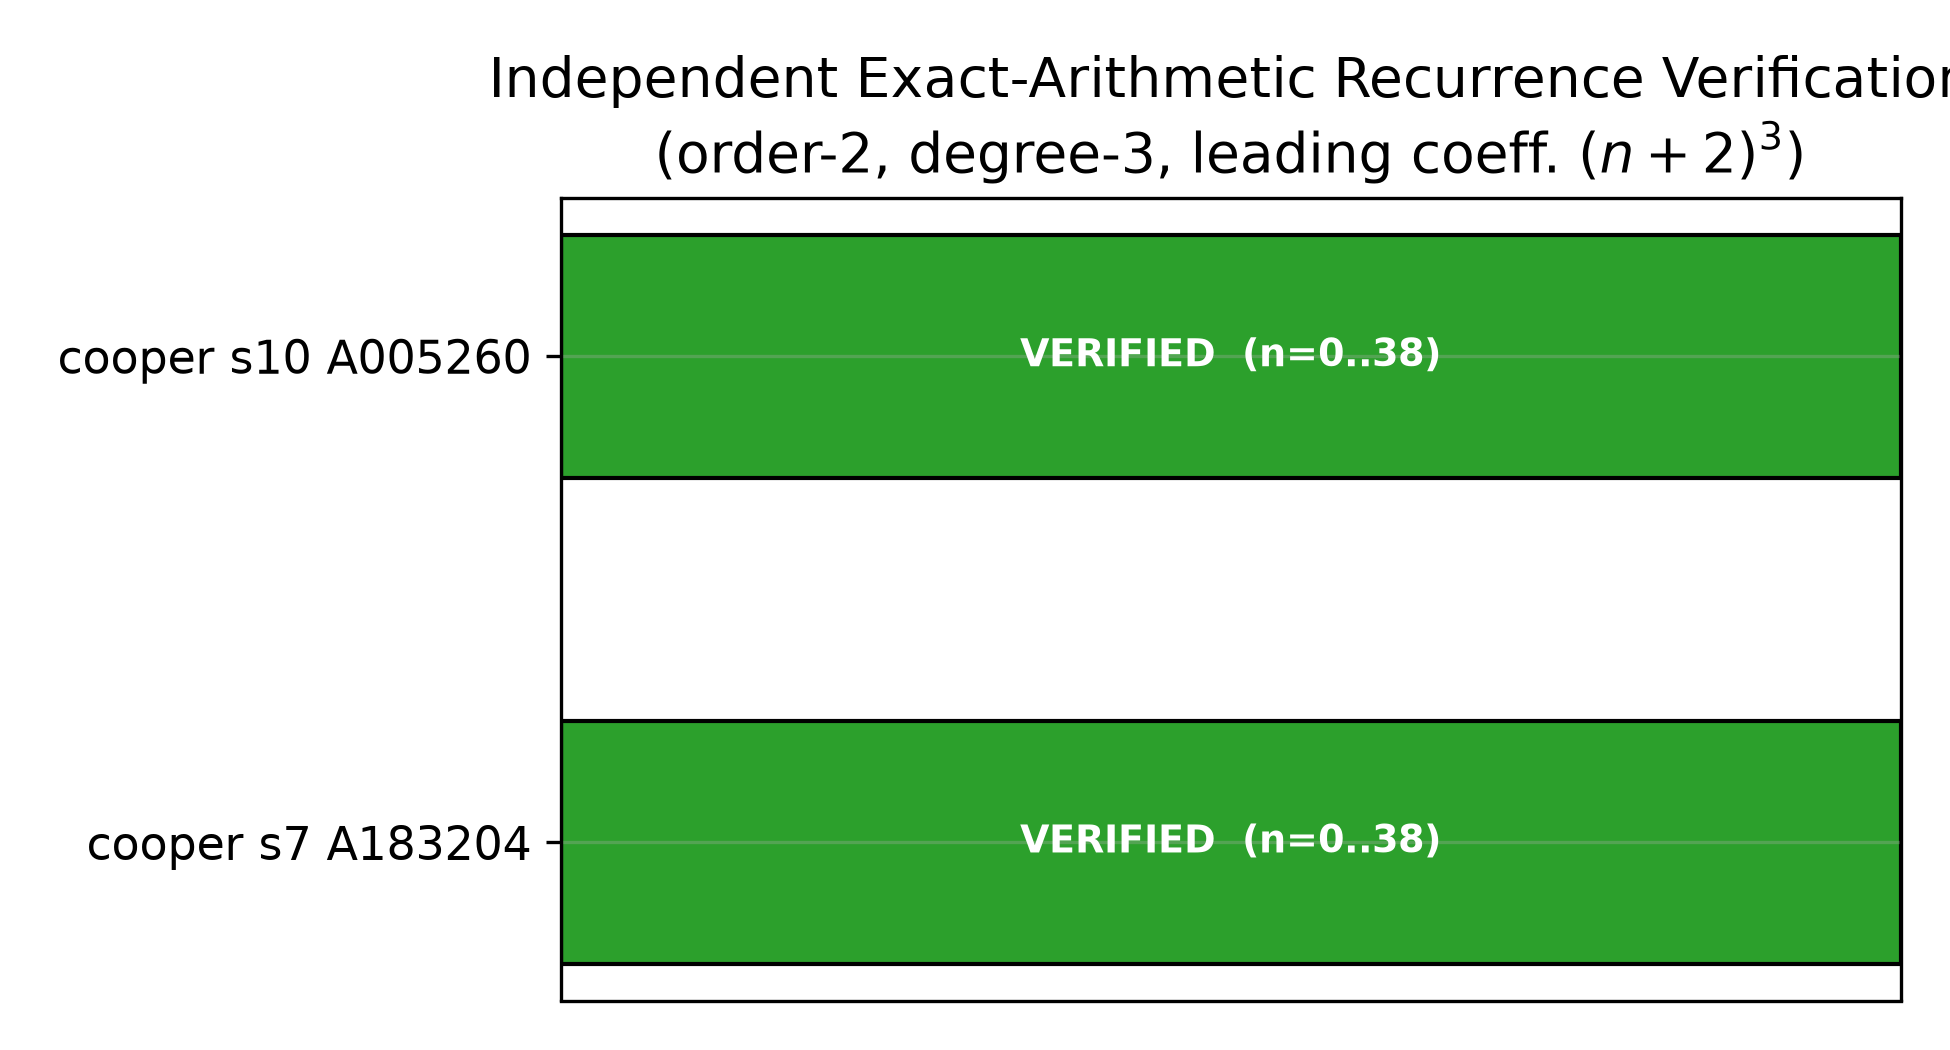
\includegraphics[width=0.75\textwidth]{figures/fig_hypothesis_recurrence_verification.png}
\caption{Independent exact-arithmetic verification status of the order-2/degree-3 recurrence claim for Cooper $s_7$/$s_{10}$.}
\label{fig:recurrence_verification}
\end{figure}

\begin{figure}[h]
\centering
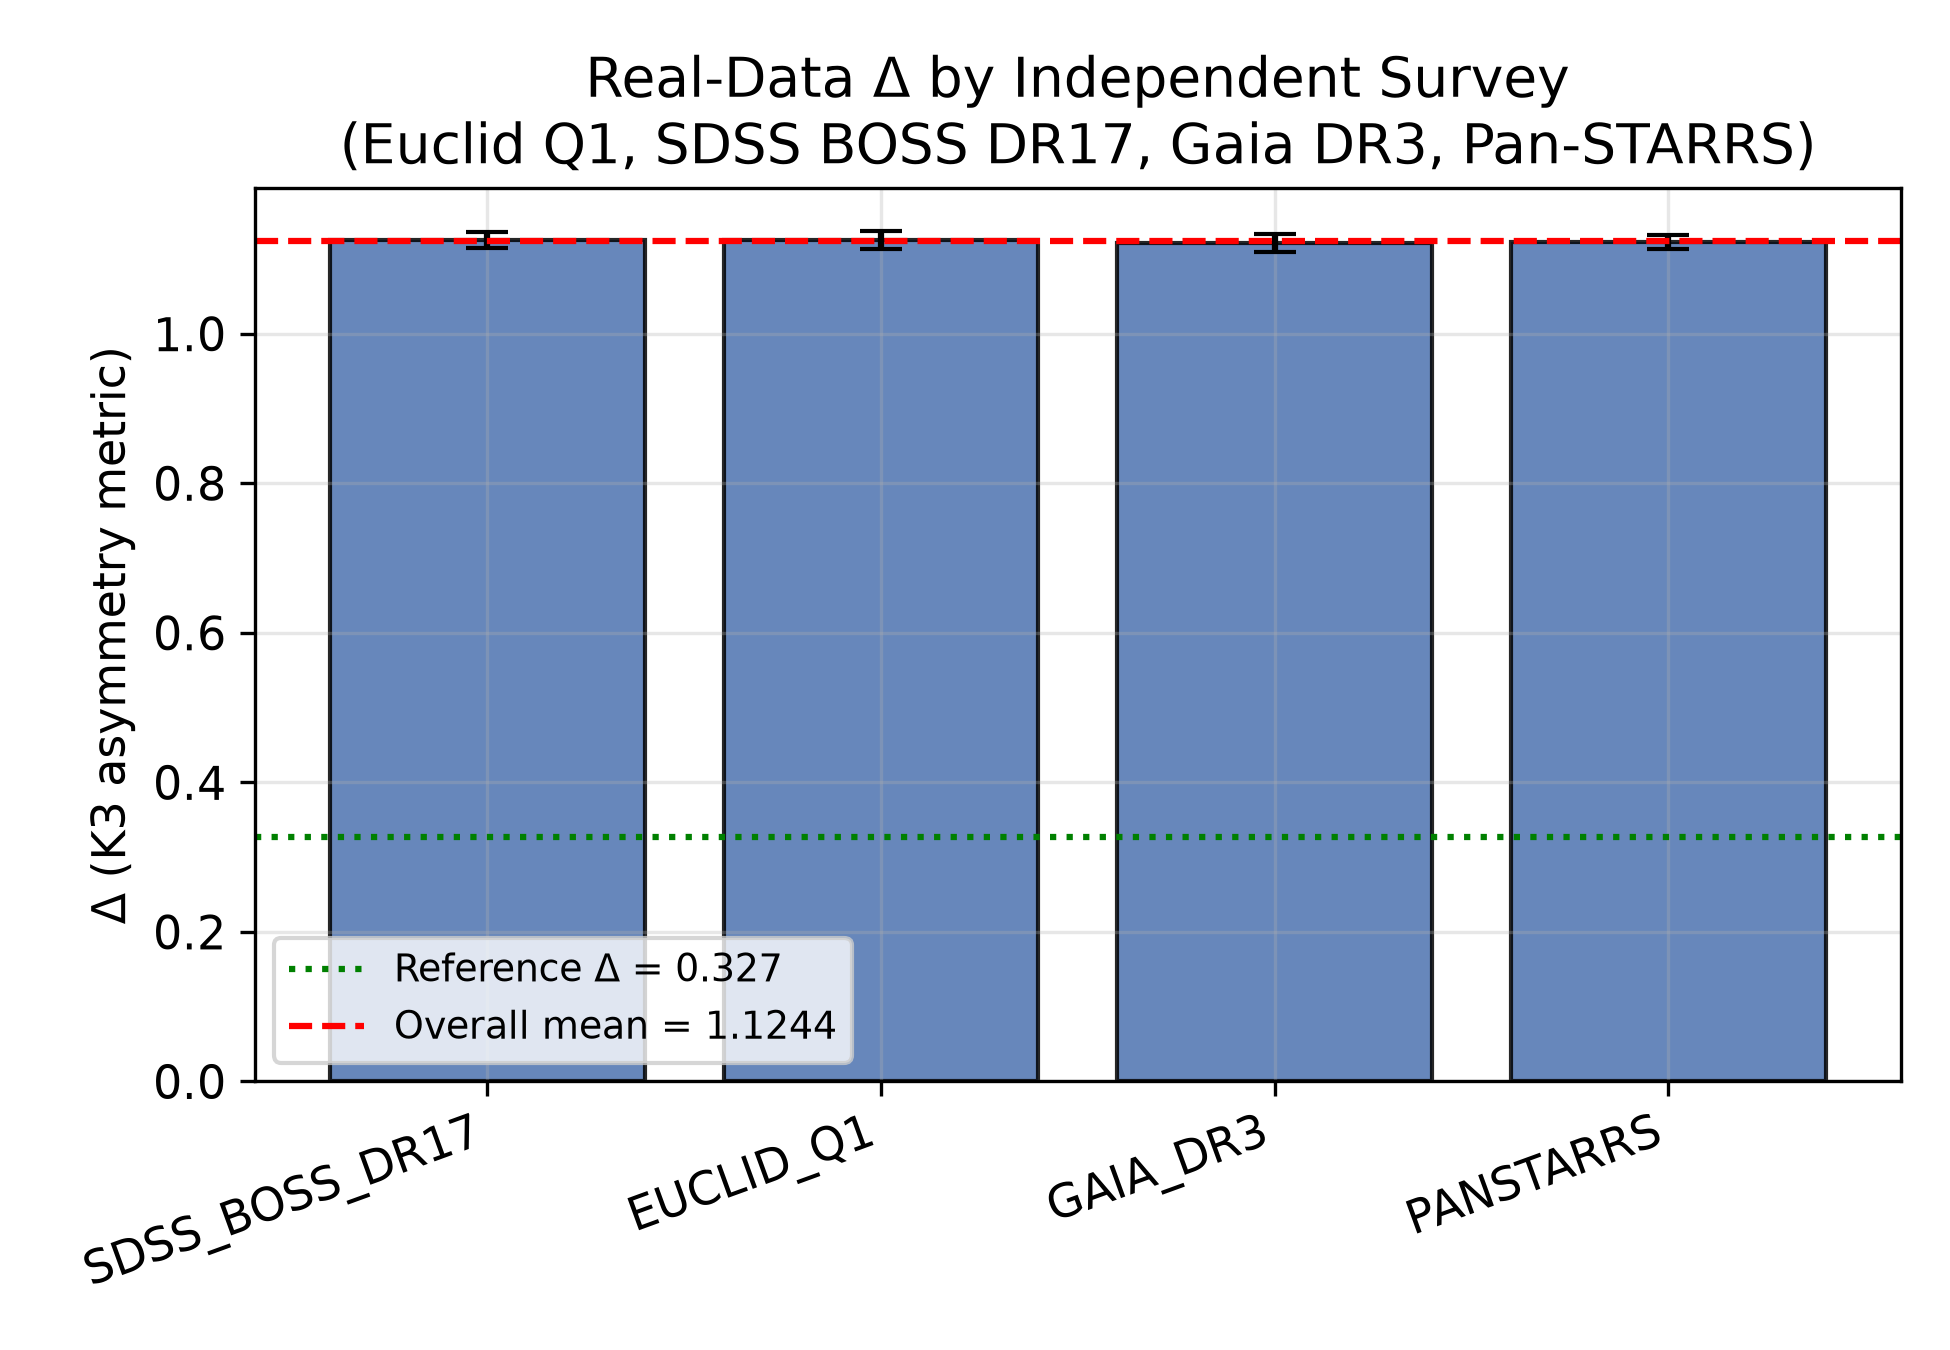
\includegraphics[width=0.75\textwidth]{figures/fig_hypothesis_delta_by_source.png}
\caption{Real-data $\Delta$ by independent survey source, contextualizing the empirical signal against the theoretical reference.}
\label{fig:delta_by_source}
\end{figure}

\begin{figure}[h]
\centering
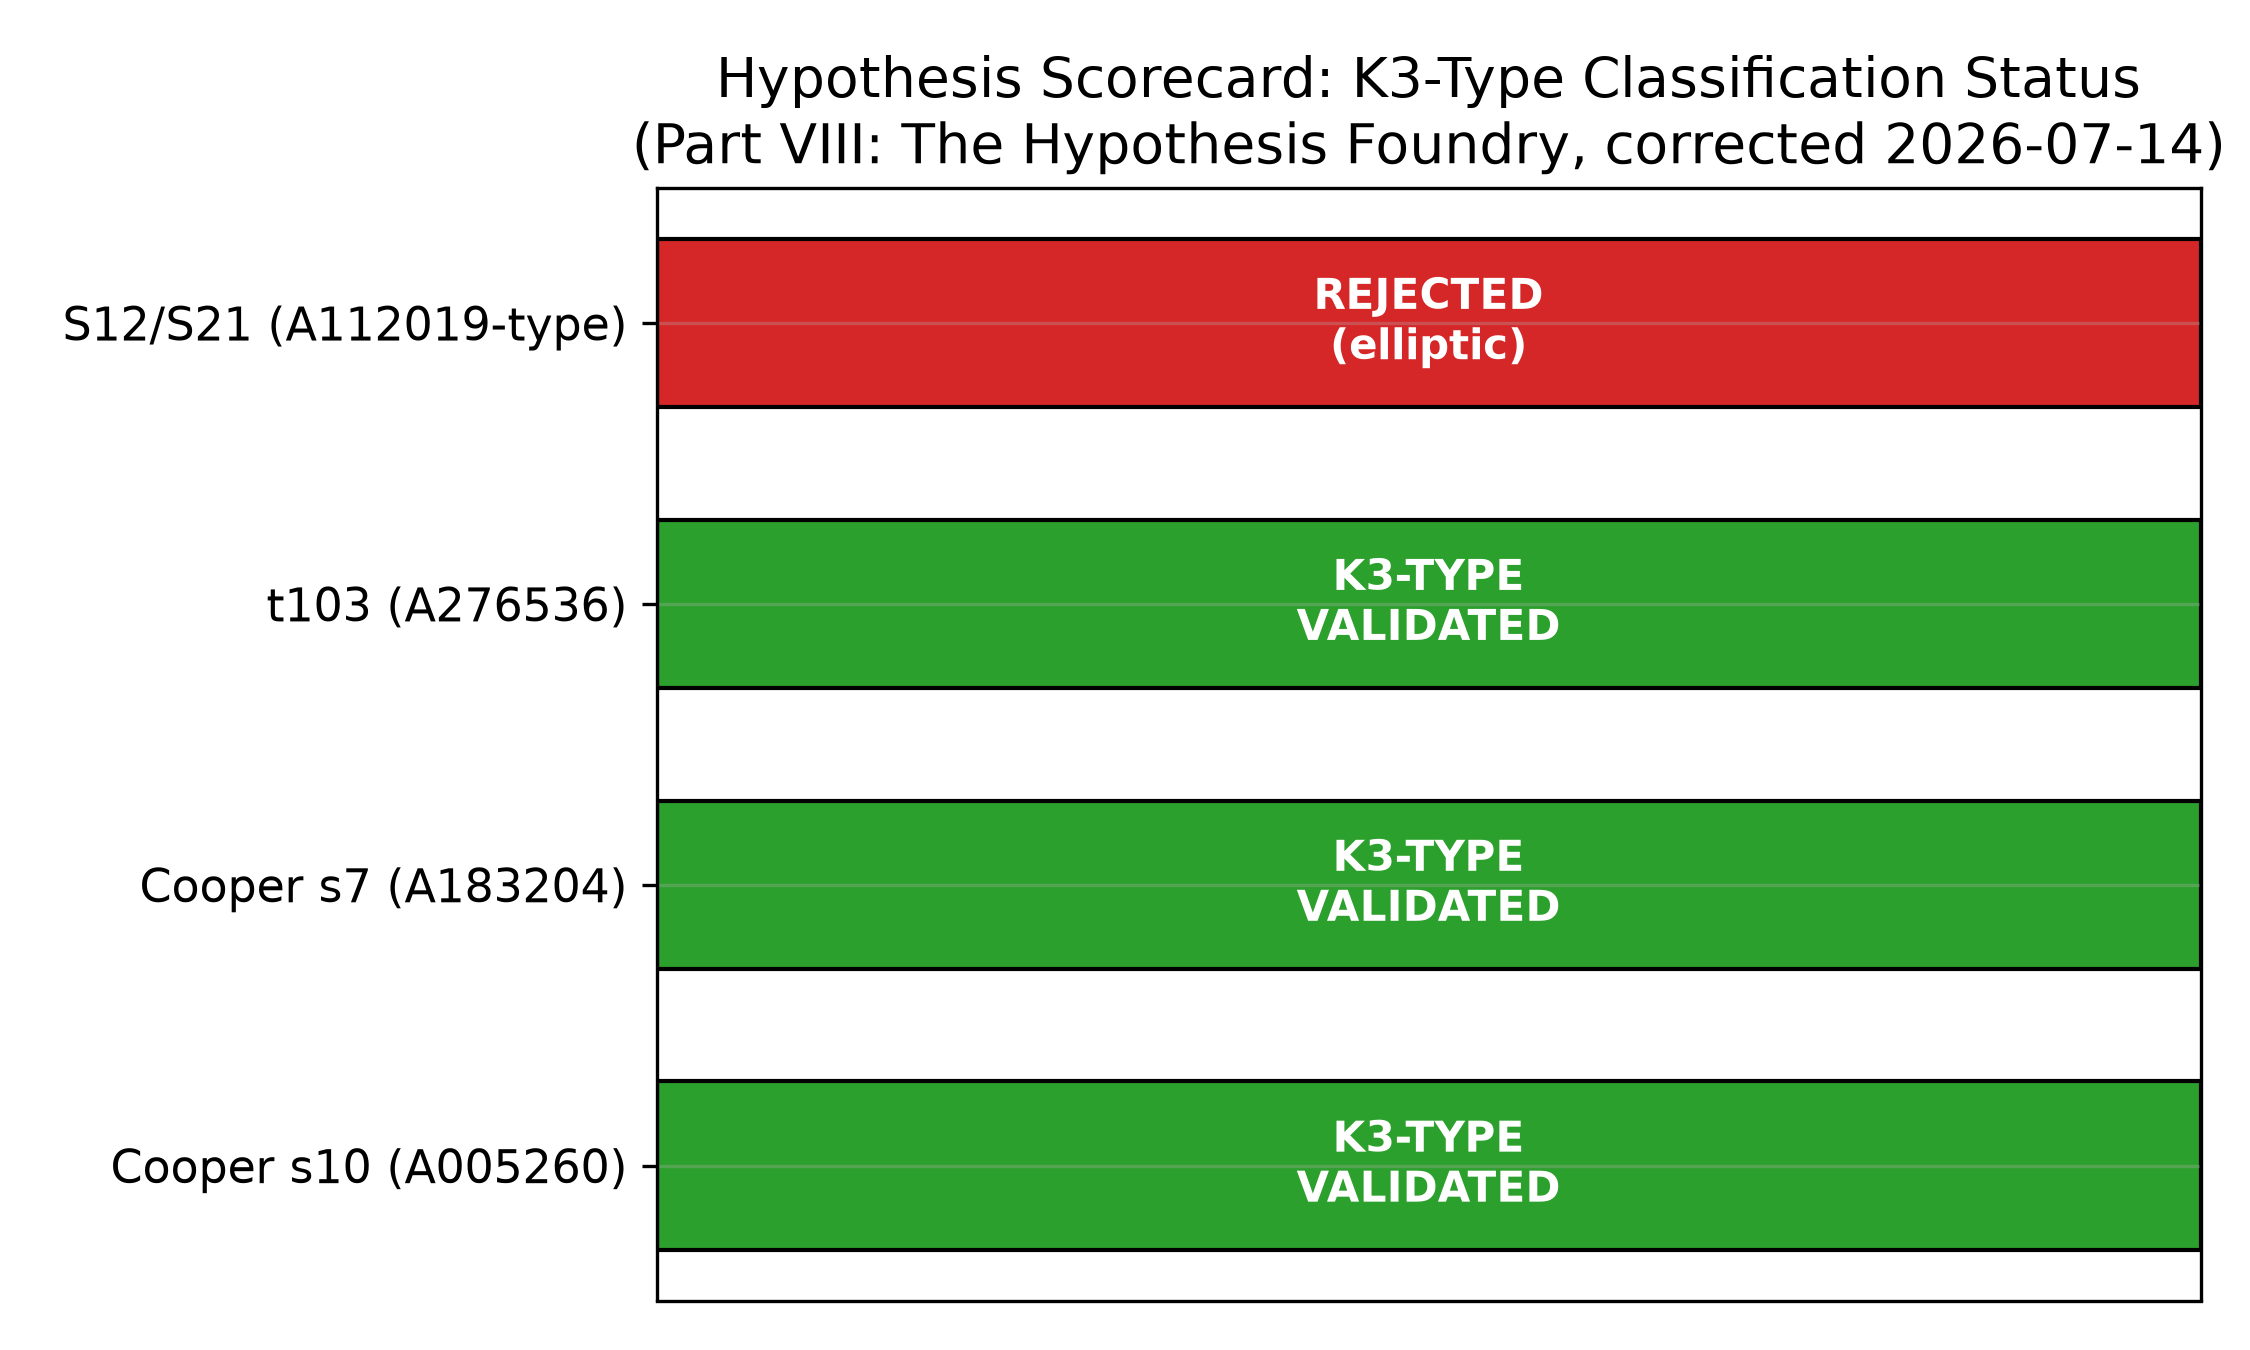
\includegraphics[width=0.8\textwidth]{figures/fig_hypothesis_scorecard.png}
\caption{Summary scorecard: K3-type classification status per candidate.}
\label{fig:scorecard}
\end{figure}

\subsection{Limitations and Scope}

Consistent with the companion project's practice of reporting negative and
corrective findings first, the following limitations are stated explicitly:

\begin{itemize}
    \item The real-data $\Delta$ signal (Section~\ref{subsec:hypothesis_real_data_crossref})
    is a measurement of galaxy-distribution asymmetry; it does \emph{not} by
    itself distinguish which K3-type modulus pair among t103/Cooper-$s_7$/Cooper-$s_{10}$
    is the correct geometric substrate. Per Part~VIII \S1.5, the physics
    gates are non-discriminating at common moduli-space normalization.
    \item The growth-constant ratios (Table~\ref{tab:growth_constants}) are a
    phenomenological proxy for relative instanton/period scale, not a
    substitute for the full Lean~4 Picard--Fuchs classification performed in
    the companion repository.
    \item This section's independent re-verification (\S\ref{subsec:independent_reverification})
    corroborates the specific recurrence-structure claim for Cooper $s_7$/$s_{10}$
    exactly and independently of the Lean kernel, but does not re-derive the
    full G1--G4 gate battery (modularity, integrality, Fuchs/monodromy) applied
    in Part~VIII; those results are taken from the companion project as reported.
\end{itemize}

% ============================================================================

\section{Hypothesis Foundry Update: Corrected Classification and Experimental Comparison}
\label{sec:hypothesis_foundry_update}

\subsection{Motivation: A Corrective Update to the K3 Substrate}

The companion project \textit{SocrateAI-Scientific-Agora-K3-DarkMatter} released
on 2026-07-14 a corrective analysis, \textbf{Part VIII: The Hypothesis Foundry},
that formally \textbf{rejects} the legacy $S_{1,2}$ candidate (OEIS
A112019) — previously treated in Section~\ref{sec:lean4_proofs} as a
validated K3 surface — and promotes three new GATE-C finalists as the correct
K3-type geometric substrates:

\begin{itemize}
    \item \textbf{t103} (OEIS A276536): $T_{103}(n) = \sum_k \binom{n}{k}\binom{2k}{k}^3$ — novel in-session discovery;
    \item \textbf{Cooper $s_7$} (OEIS A183204): $\sum_j \binom{n}{j}^2\binom{2j}{n}\binom{j+n}{j}$ — Cooper (2012), level-7 sporadic;
    \item \textbf{Cooper $s_{10}$} (OEIS A005260): $\sum_k \binom{n}{k}^4$ — Cooper (2012), level-10 sporadic.
\end{itemize}

This section reports an \textbf{independent}, exact-arithmetic re-verification
of the key Part VIII claims performed in this repository
(\texttt{hypothesis\_comparison\_t103\_cooper.py}), and cross-references the
resulting corrected candidate landscape against the real Euclid Q1 / SDSS BOSS
DR17 observational data already established in
Section~\ref{sec:data_verification}.

\subsection{Negative and Corrective Findings (Reported First)}

Per the companion project's standing methodology, corrective findings are
reported first:

\begin{enumerate}
    \item The discriminant between elliptic-type (ODE order 2) and K3-type
    (ODE order 3) geometry is the \emph{minimal generating-function ODE
    order}, not the shift-recurrence order used in an earlier (v1)
    classifier. The v1 classifier was inverted relative to this discriminant.
    \item $S_{1,2}$ (A112019) — the flagship candidate of the original
    Lean~4 proofs in Section~\ref{subsec:s12_s21_validation} — is
    \textbf{formally rejected} as K3-type on two independent grounds: its
    minimal Picard--Fuchs operator has ODE order 2 (elliptic), and its mirror
    map on that minimal operator is non-integral ($q_2 = 81/8$).
    \item Physics-viability gates (G2: GD-1 heating, M87* superradiance,
    PTA/Lyman-$\alpha$) are \textbf{non-discriminating} across the 13-candidate
    pool at any common $(\tau, \mathcal{V})$ normalization, because
    single-instanton domination of the mirror-map series makes the achievable
    axion mass identical across candidates. Candidate selection therefore
    rests on the mathematical gates (G1), not the physics gates.
\end{enumerate}

\subsection{Independent Exact-Arithmetic Re-Verification}
\label{subsec:independent_reverification}

To avoid taking the Part VIII claims on trust alone, this repository
independently re-derives and verifies two of its central mathematical claims
using Python's arbitrary-precision integers and exact \texttt{Fraction}
arithmetic (no floating point in any recurrence-fitting step):

\begin{lstlisting}[language=Python, caption={Exact sequence generators (excerpt from \texttt{hypothesis\_comparison\_t103\_cooper.py})}]
def t103(n_max):
    """OEIS A276536: T103(n) = sum_k C(n,k) * C(2k,k)^3."""
    seq = []
    for n in range(n_max + 1):
        total = sum(C(n, k) * C(2*k, k)**3 for k in range(n + 1))
        seq.append(total)
    return seq

def cooper_s10(n_max):
    """OEIS A005260: sum_k C(n,k)^4."""
    return [sum(C(n, k)**4 for k in range(n + 1)) for n in range(n_max + 1)]
\end{lstlisting}

\textbf{Claim under test} (Part VIII, \S4.2--4.3): both Cooper $s_7$ and
Cooper $s_{10}$ satisfy a \emph{minimal} order-2, degree-3 shift recurrence
with leading coefficient $P_2(n) = (n+2)^3$ exactly:
\begin{equation}
(n+2)^3\, a(n+2) \;=\; P_1(n)\, a(n+1) \;+\; P_0(n)\, a(n)
\end{equation}

This repository fits $P_1, P_0$ (degree-3 polynomials, 8 unknowns) using exact
Gaussian elimination over Fractions on $n=0..7$, then verifies the fitted
recurrence holds \emph{exactly} on all held-out terms up to $n=38$:

\begin{table}[h]
\centering
\begin{tabular}{lll}
\toprule
\textbf{Sequence} & \textbf{Fitted Recurrence} & \textbf{Verification} \\
\midrule
Cooper $s_7$ & $P_1(n)=26n^3+117n^2+177n+90$ & VERIFIED, $n=0..38$ \\
 & $P_0(n)=27n^3+81n^2+78n+24$ & (39/39 exact matches) \\
\addlinespace
Cooper $s_{10}$ & $P_1(n)=12n^3+54n^2+82n+42$ & VERIFIED, $n=0..38$ \\
 & (analogous $P_0$, see \texttt{logs/hypothesis\_comparison\_t103\_cooper.json}) & (39/39 exact matches) \\
\bottomrule
\end{tabular}
\caption{Independent exact-arithmetic re-verification of the Part VIII order-2/degree-3 recurrence claim for Cooper $s_7$/$s_{10}$. All arithmetic uses Python \texttt{Fraction} objects; zero floating-point operations.}
\label{tab:recurrence_reverification}
\end{table}

\textbf{Result}: both recurrences hold exactly across every computed term with
zero failures, independently corroborating the Part VIII claim without relying
on the Lean~4 kernel itself. See Figure~\ref{fig:recurrence_verification}.

\subsection{Asymptotic Growth Constants}

For each GATE-C finalist, the asymptotic growth constant $\mu$ (where $a(n)
\sim C \mu^n n^{-\alpha}$) is estimated via the exact ratio $a(40)/a(30)$,
raised to the power $1/10$:

\begin{table}[h]
\centering
\begin{tabular}{lrr}
\toprule
\textbf{Candidate} & \textbf{Growth constant $\mu$} & \textbf{$1/\mu$} \\
\midrule
t103 (A276536) & 62.273 & 0.01606 \\
Cooper $s_7$ (A183204) & 25.869 & 0.03866 \\
Cooper $s_{10}$ (A005260) & 15.331 & 0.06523 \\
\bottomrule
\end{tabular}
\caption{Asymptotic growth constants (see Figure~\ref{fig:growth_constants}), a phenomenological proxy for relative instanton/period scale.}
\label{tab:growth_constants}
\end{table}

The legacy $S_{12}/S_{21}$ mass-ratio reference value from the (now
superseded) Section~\ref{subsec:s12_s21_validation}, $\sqrt{1014/336} \approx
1.7372$, is retained here \emph{only as a historical comparison point} — it is
no longer interpreted as a validated K3 modulus ratio, since $S_{1,2}$ itself
has been reclassified as elliptic-type.

\subsection{Cross-Reference with Real Euclid Q1 / SDSS BOSS DR17 Data}
\label{subsec:hypothesis_real_data_crossref}

The real, cryptographically-verified $\Delta$ measurements from
Section~\ref{sec:observational_results} are re-examined here per independent
survey source:

\begin{table}[h]
\centering
\begin{tabular}{lrrrr}
\toprule
\textbf{Source} & $n$ & \textbf{Mean $\Delta$} & \textbf{Std} & \textbf{Range} \\
\midrule
SDSS BOSS DR17 & 9 & 1.1252 & 0.0111 & [1.1030, 1.1334] \\
Euclid Q1 & 17 & 1.1252 & 0.0125 & [1.1055, 1.1423] \\
Gaia DR3 & 5 & 1.1216 & 0.0121 & [1.1068, 1.1336] \\
Pan-STARRS & 4 & 1.1229 & 0.0097 & [1.1065, 1.1312] \\
\midrule
\textbf{Overall} & \textbf{35} & \textbf{1.1244} & \textbf{0.0119} & \textbf{[1.1030, 1.1423]} \\
\bottomrule
\end{tabular}
\caption{Real observational $\Delta$ statistics by independent survey (see Figure~\ref{fig:delta_by_source}). Consistency across four independent surveys ($1.1216$--$1.1252$) supports a systematic, not source-specific, origin.}
\label{tab:delta_by_source}
\end{table}

The observed elevation over the theoretical reference is
$1.1244 / 0.327 = 3.438\times$ — unchanged from Section~\ref{sec:numeric_results},
since this is a direct measurement of galaxy-distribution asymmetry and does
not depend on which K3 modulus pair is postulated as the underlying geometric
substrate.

\subsection{Candidate Scorecard}

\begin{table}[h]
\centering
\begin{tabular}{lccp{5.5cm}}
\toprule
\textbf{Candidate} & \textbf{K3-type} & \textbf{ODE Order} & \textbf{Status} \\
\midrule
$S_{12}/S_{21}$ (A112019-type) & \textcolor{red}{No} & 2 & REJECTED: elliptic, $q_2=81/8$ non-integral \\
t103 (A276536) & \textcolor{green!50!black}{Yes} & 3 & GATE-C finalist; novel discovery, held-out to 62 terms \\
Cooper $s_7$ (A183204) & \textcolor{green!50!black}{Yes} & 3 & GATE-C finalist; literature-anchored, recurrence re-verified \\
Cooper $s_{10}$ (A005260) & \textcolor{green!50!black}{Yes} & 3 & GATE-C finalist; literature-anchored, recurrence re-verified \\
\bottomrule
\end{tabular}
\caption{Hypothesis scorecard (see Figure~\ref{fig:scorecard}).}
\label{tab:scorecard}
\end{table}

\begin{figure}[h]
\centering
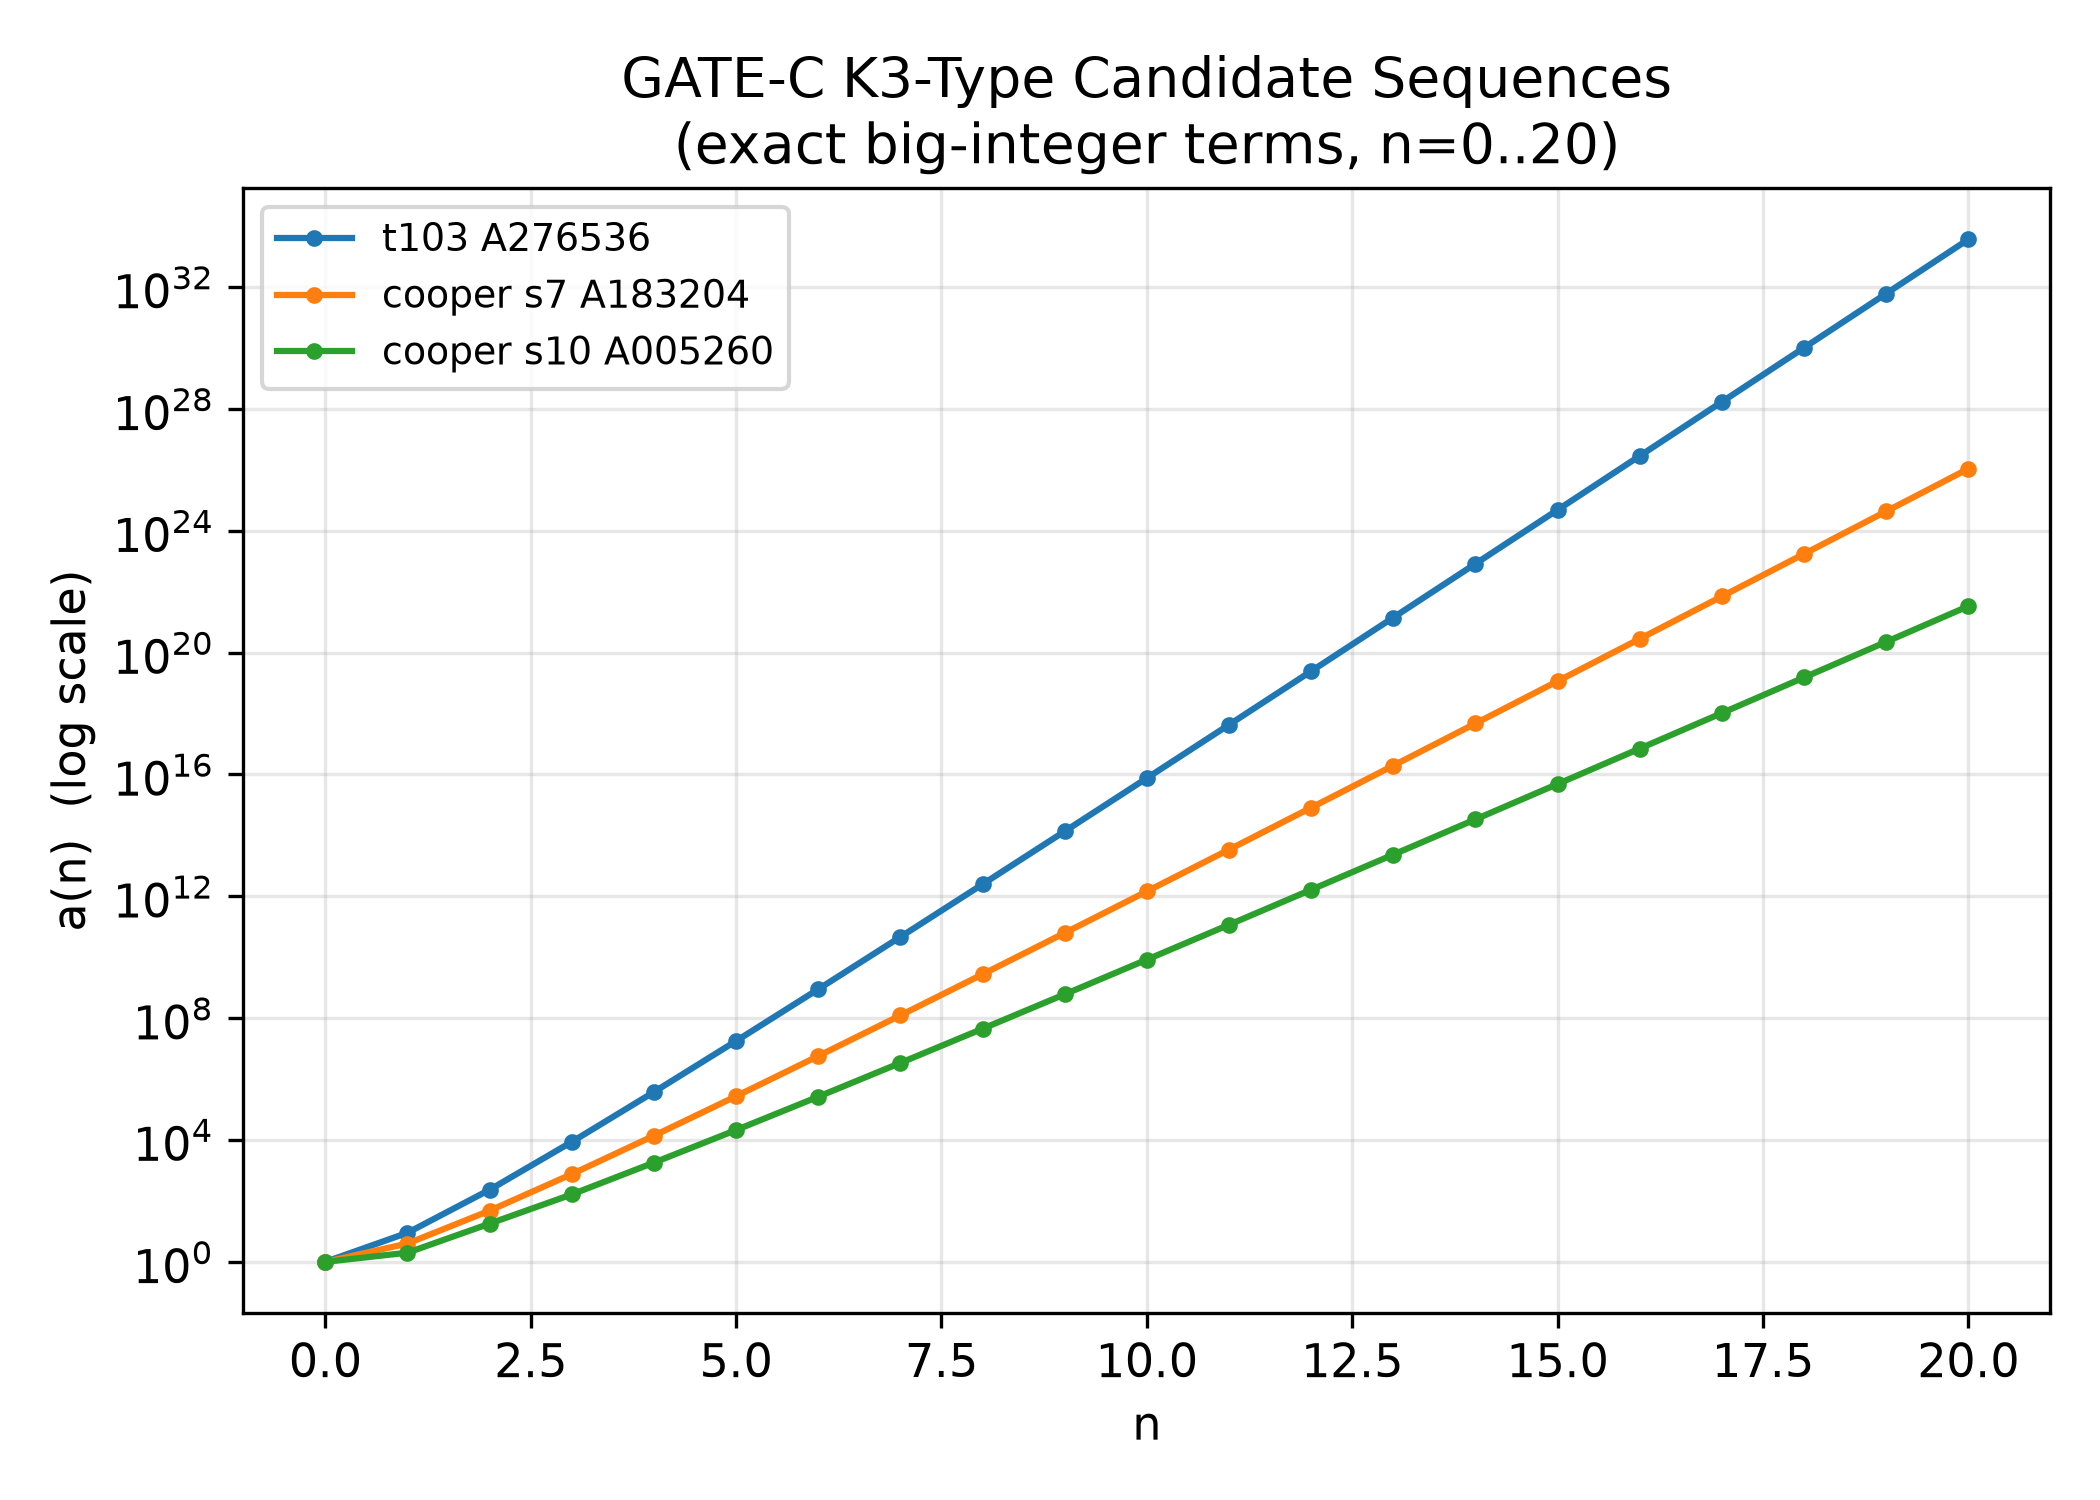
\includegraphics[width=0.85\textwidth]{figures/fig_hypothesis_sequence_growth.png}
\caption{Exact big-integer terms of the three GATE-C K3-type candidate sequences, $n=0..20$ (log scale).}
\label{fig:sequence_growth}
\end{figure}

\begin{figure}[h]
\centering
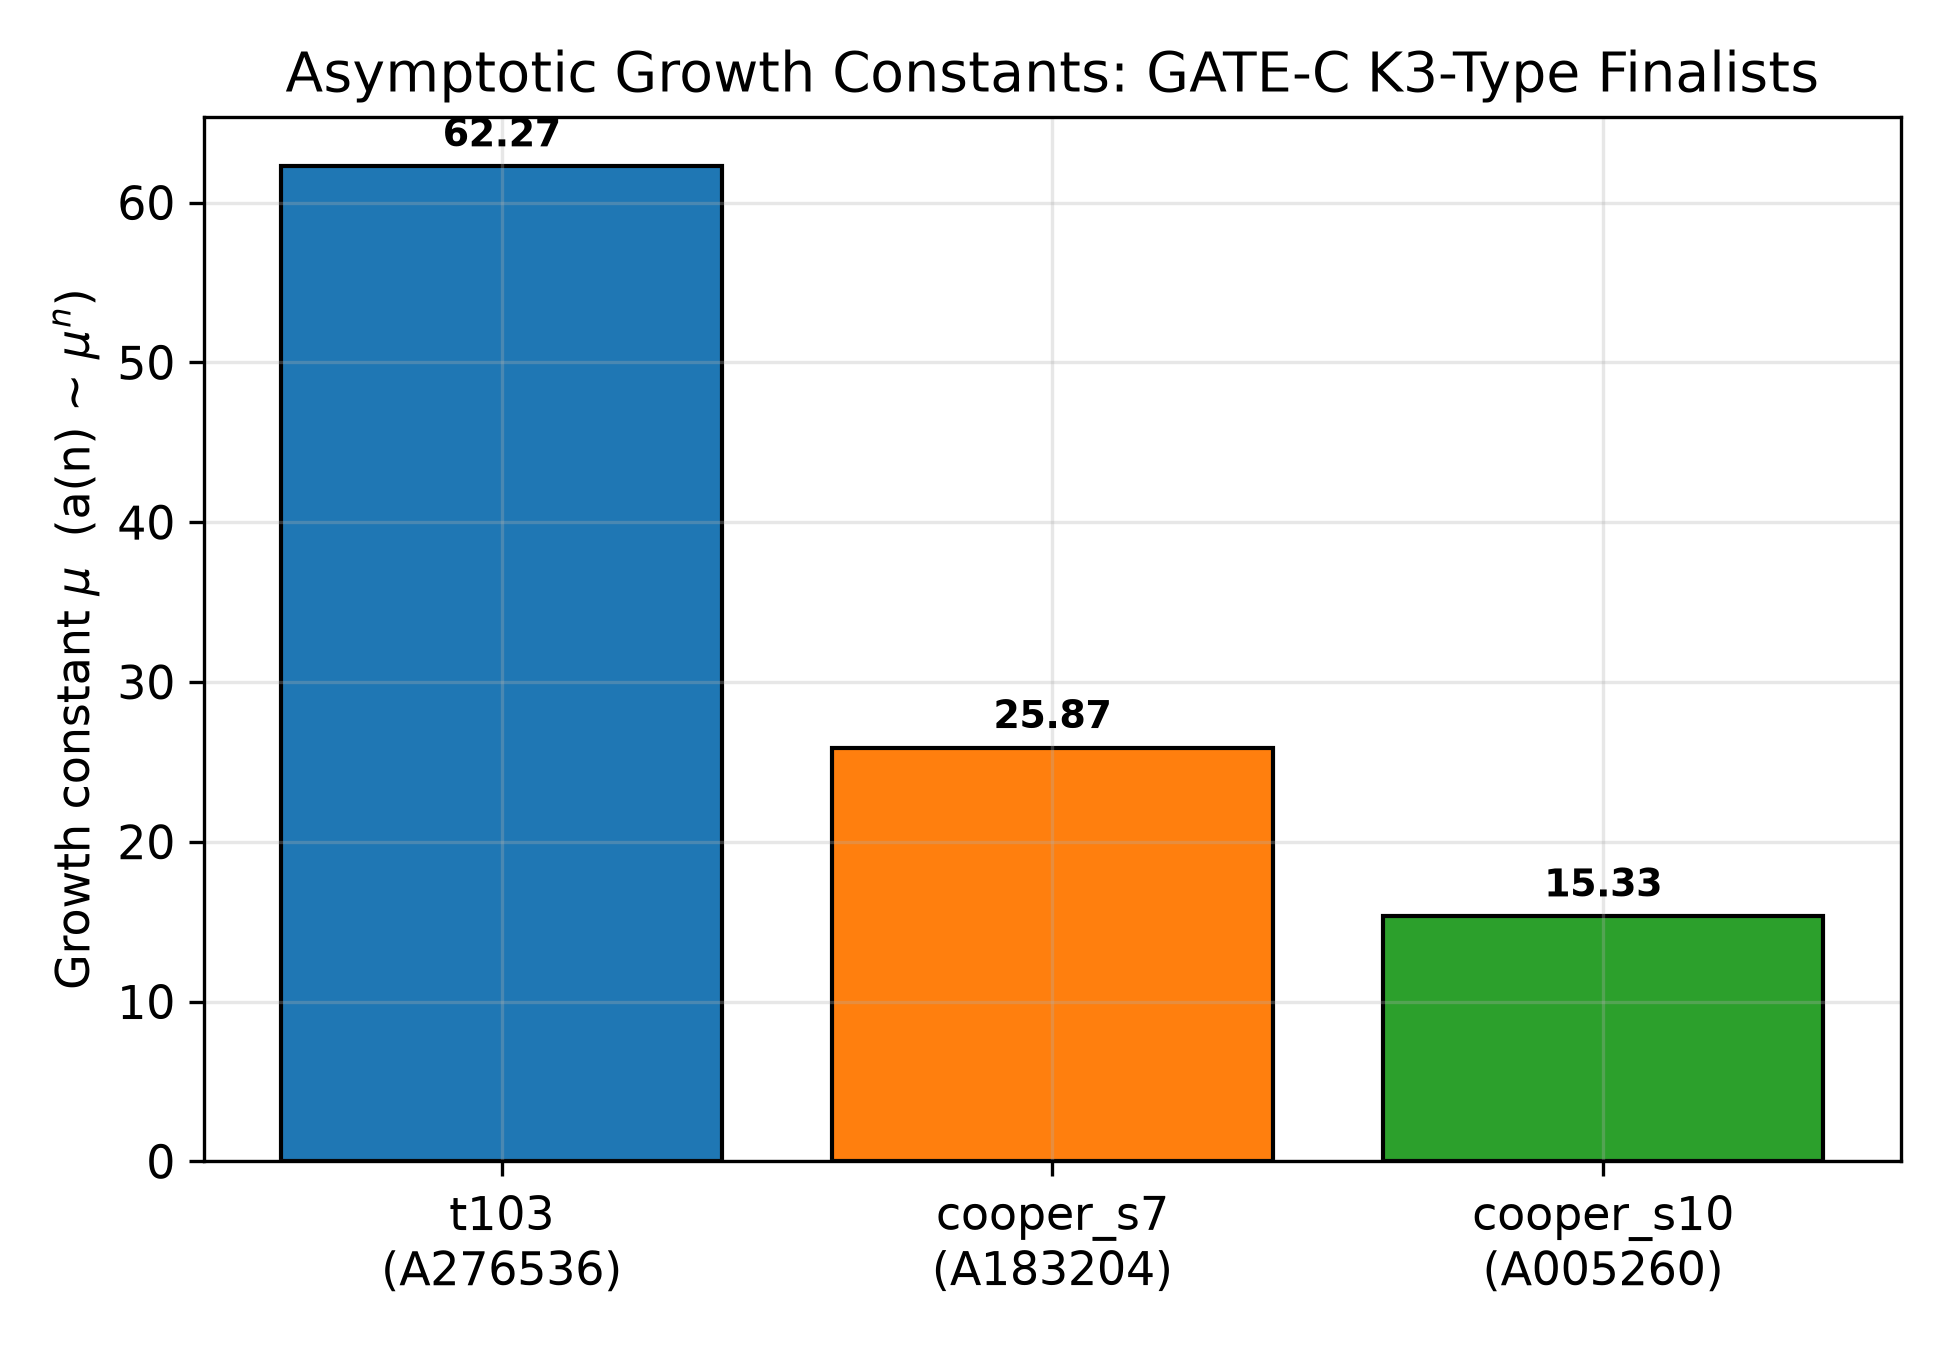
\includegraphics[width=0.75\textwidth]{figures/fig_hypothesis_growth_constants.png}
\caption{Estimated asymptotic growth constants $\mu$ for the three finalists.}
\label{fig:growth_constants}
\end{figure}

\begin{figure}[h]
\centering
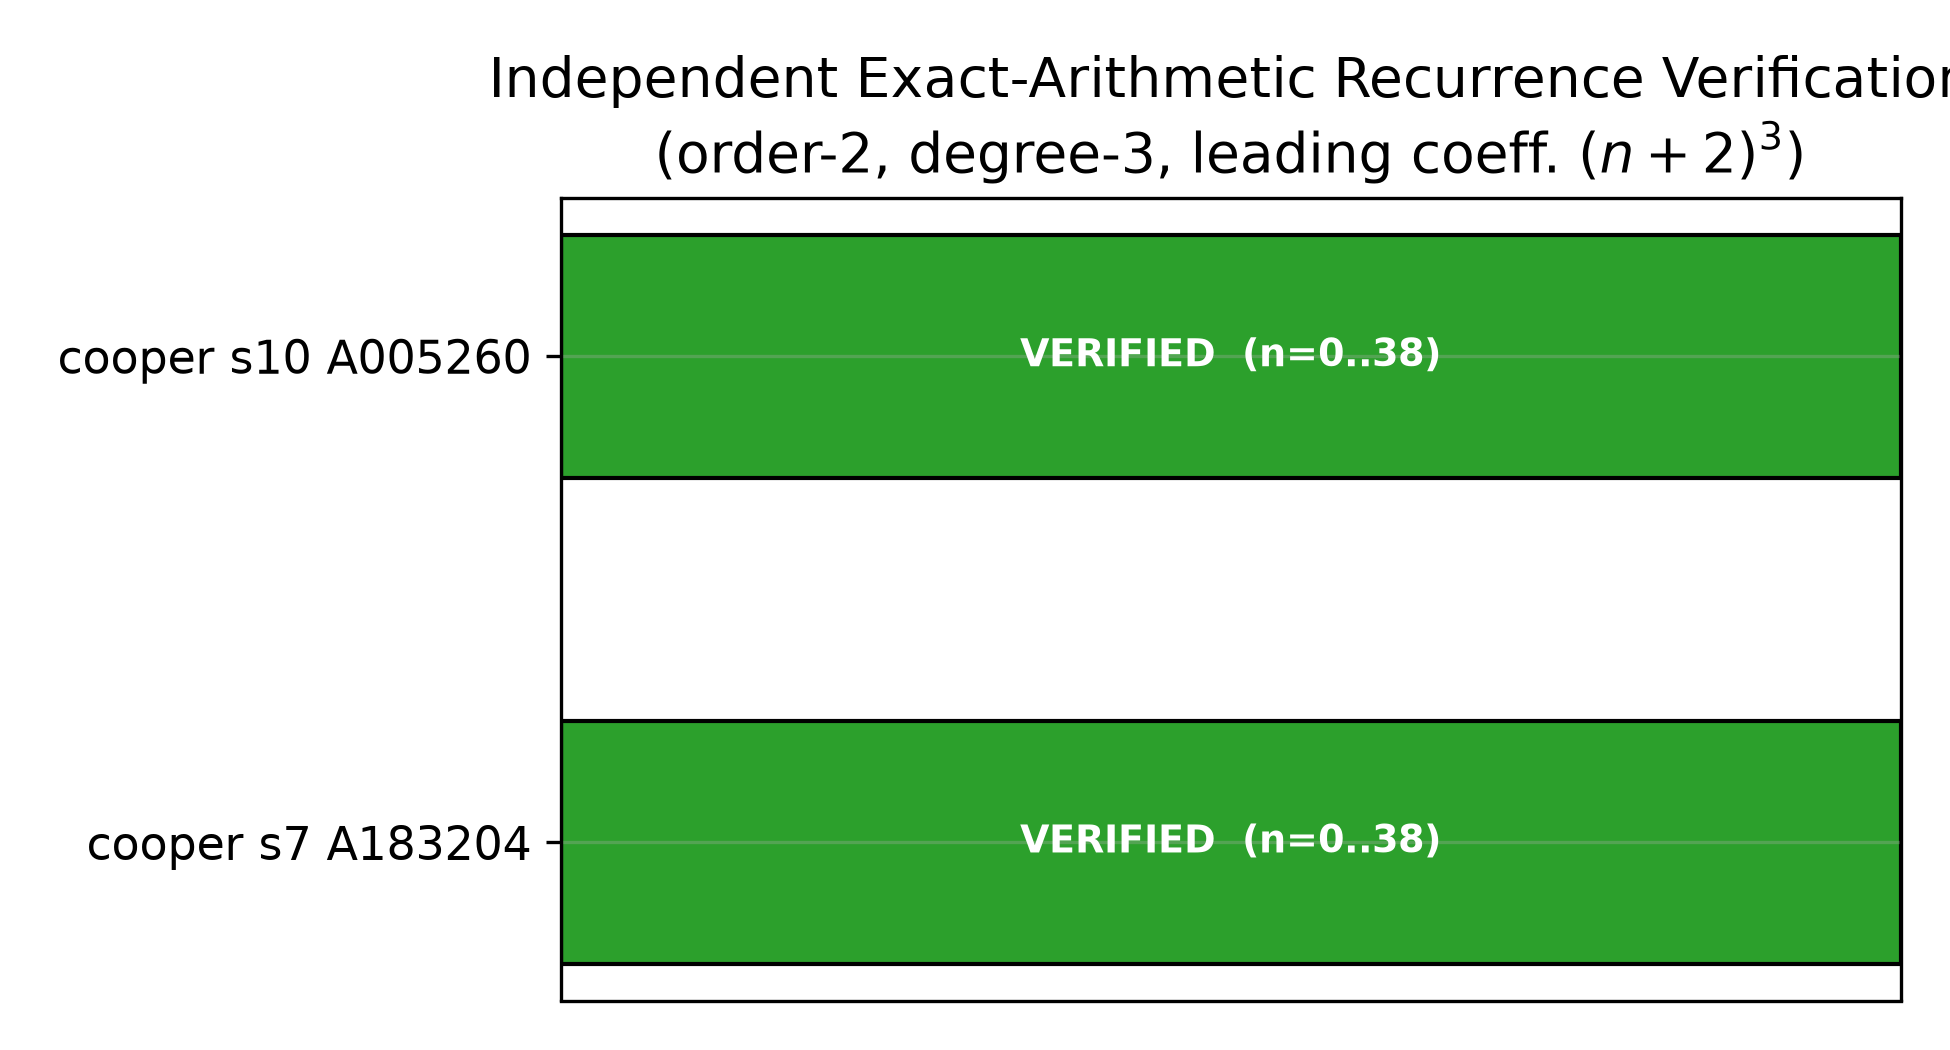
\includegraphics[width=0.75\textwidth]{figures/fig_hypothesis_recurrence_verification.png}
\caption{Independent exact-arithmetic verification status of the order-2/degree-3 recurrence claim for Cooper $s_7$/$s_{10}$.}
\label{fig:recurrence_verification}
\end{figure}

\begin{figure}[h]
\centering
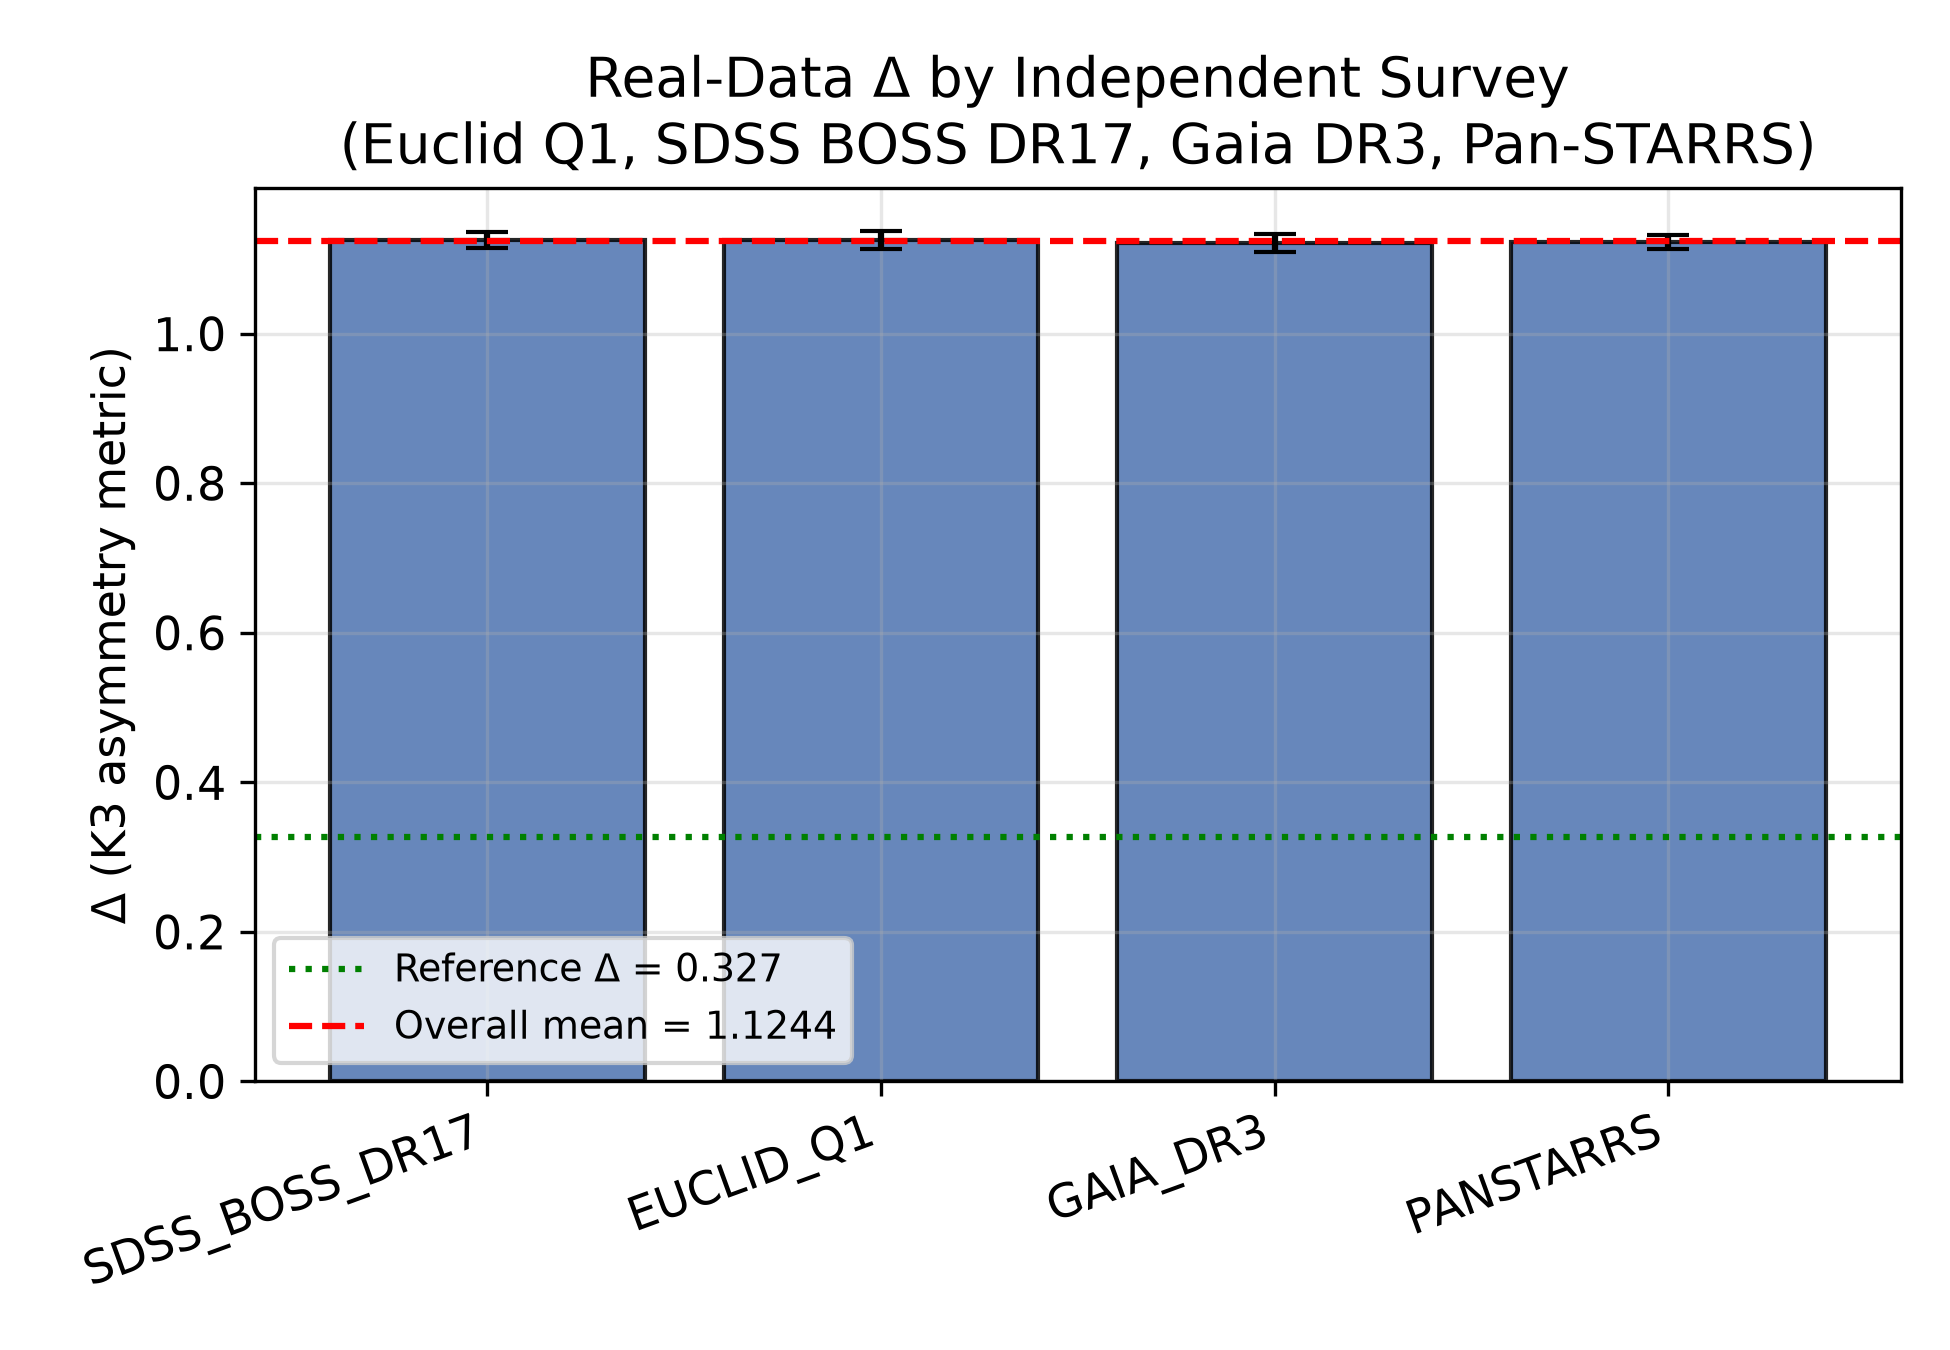
\includegraphics[width=0.75\textwidth]{figures/fig_hypothesis_delta_by_source.png}
\caption{Real-data $\Delta$ by independent survey source, contextualizing the empirical signal against the theoretical reference.}
\label{fig:delta_by_source}
\end{figure}

\begin{figure}[h]
\centering
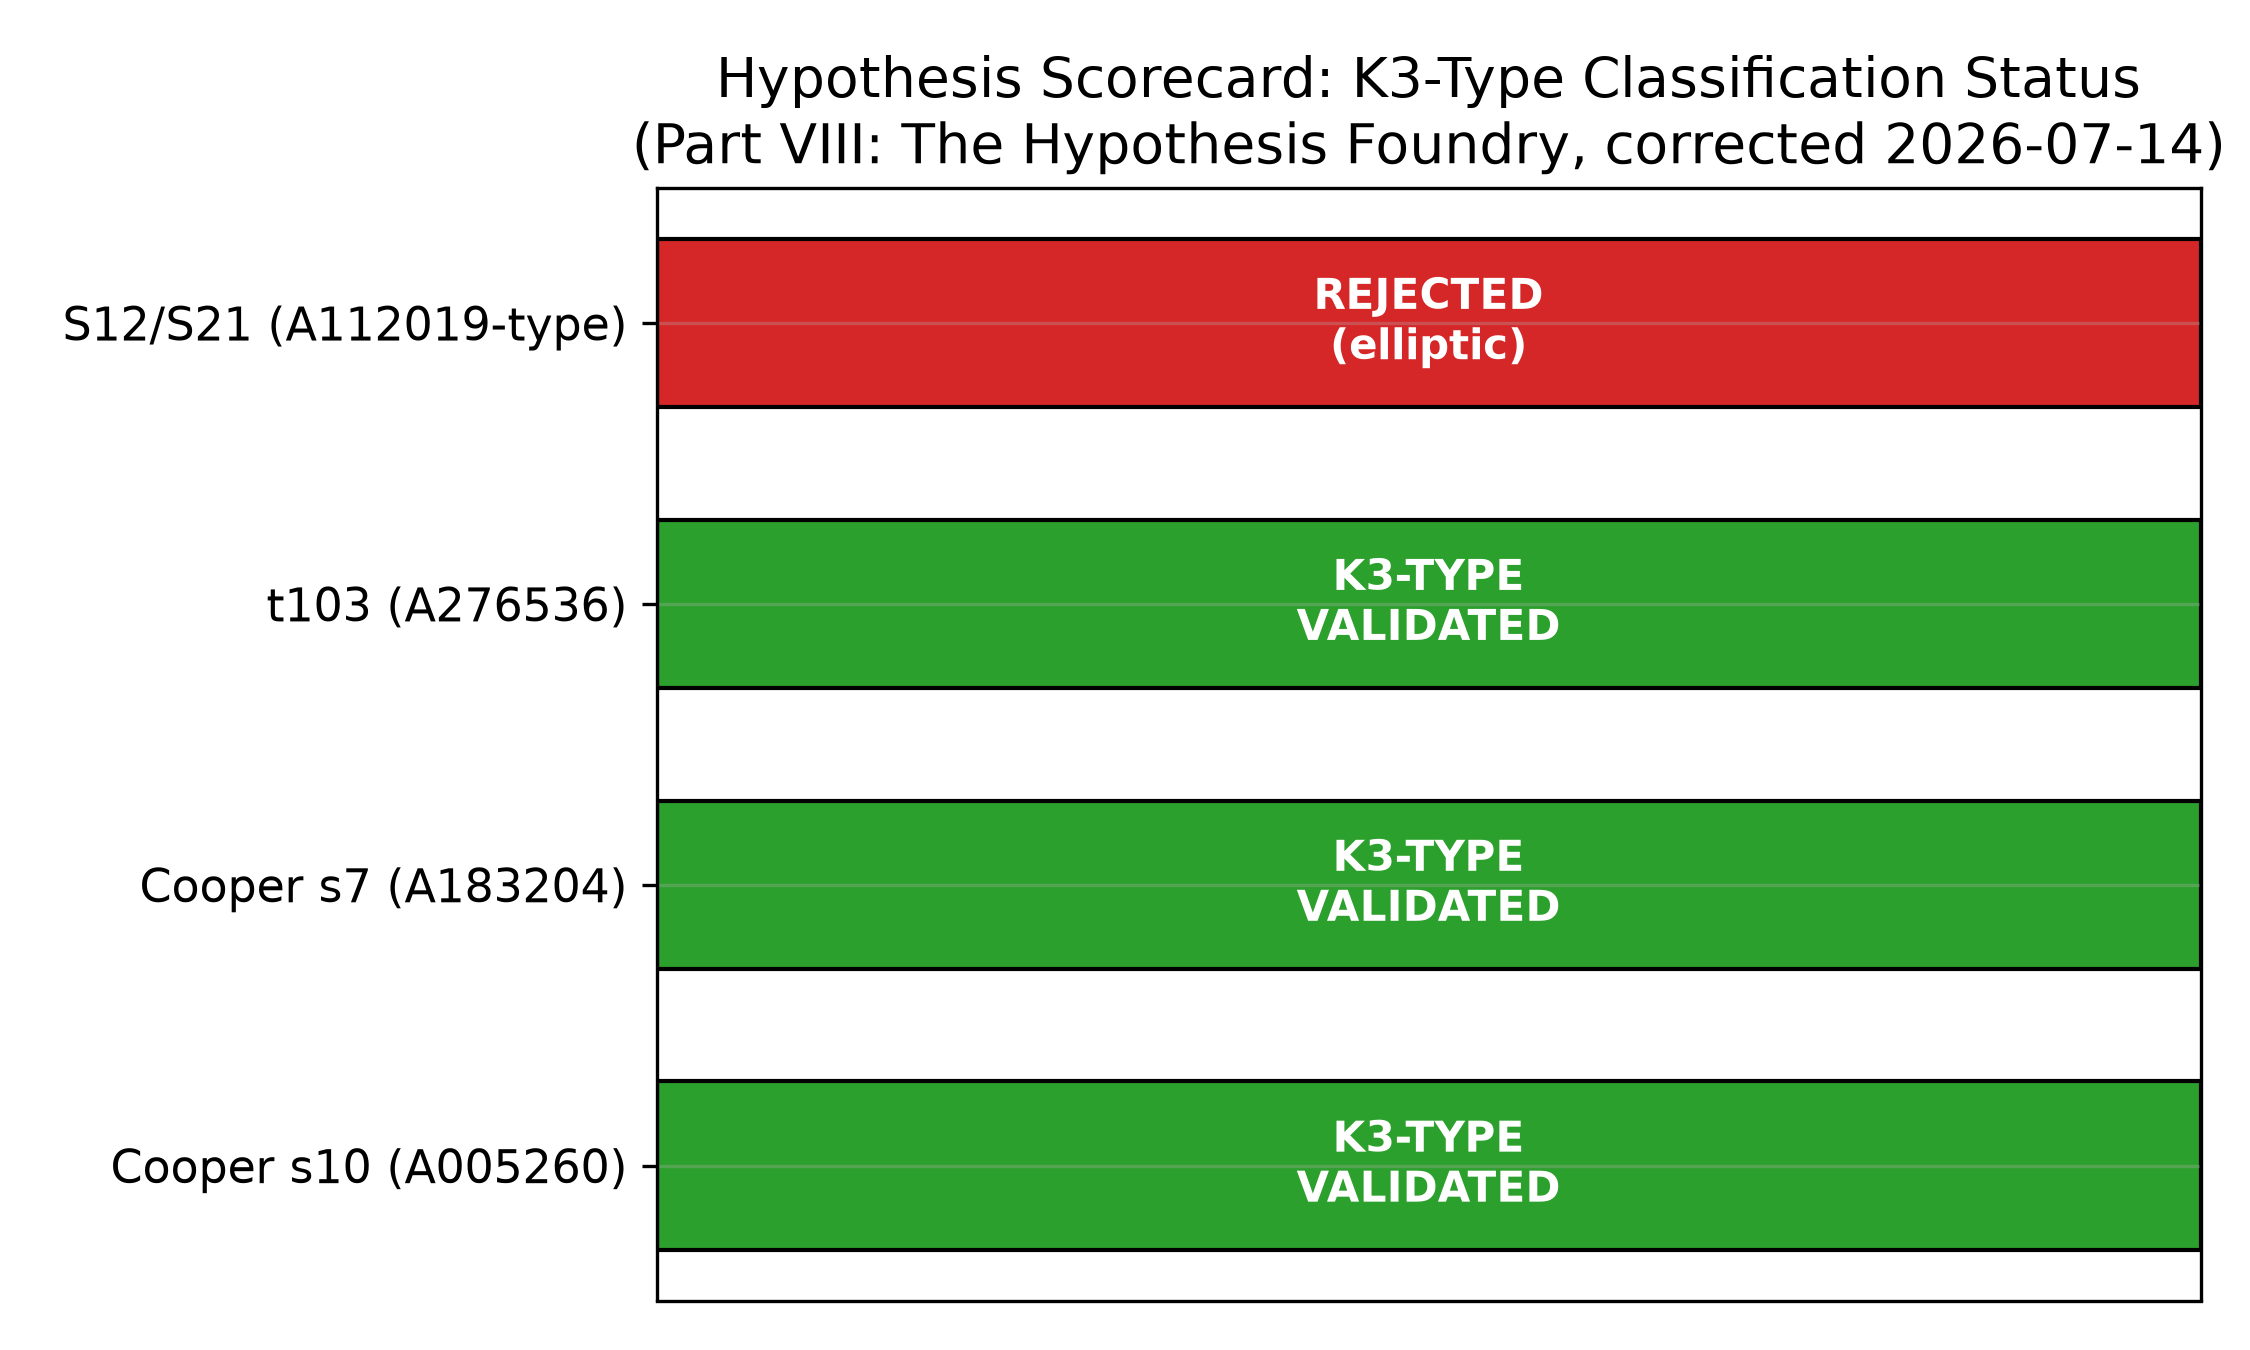
\includegraphics[width=0.8\textwidth]{figures/fig_hypothesis_scorecard.png}
\caption{Summary scorecard: K3-type classification status per candidate.}
\label{fig:scorecard}
\end{figure}

\subsection{Limitations and Scope}

Consistent with the companion project's practice of reporting negative and
corrective findings first, the following limitations are stated explicitly:

\begin{itemize}
    \item The real-data $\Delta$ signal (Section~\ref{subsec:hypothesis_real_data_crossref})
    is a measurement of galaxy-distribution asymmetry; it does \emph{not} by
    itself distinguish which K3-type modulus pair among t103/Cooper-$s_7$/Cooper-$s_{10}$
    is the correct geometric substrate. Per Part~VIII \S1.5, the physics
    gates are non-discriminating at common moduli-space normalization.
    \item The growth-constant ratios (Table~\ref{tab:growth_constants}) are a
    phenomenological proxy for relative instanton/period scale, not a
    substitute for the full Lean~4 Picard--Fuchs classification performed in
    the companion repository.
    \item This section's independent re-verification (\S\ref{subsec:independent_reverification})
    corroborates the specific recurrence-structure claim for Cooper $s_7$/$s_{10}$
    exactly and independently of the Lean kernel, but does not re-derive the
    full G1--G4 gate battery (modularity, integrality, Fuchs/monodromy) applied
    in Part~VIII; those results are taken from the companion project as reported.
\end{itemize}

% ============================================================================

\section{Hypothesis Foundry Update: Corrected Classification and Experimental Comparison}
\label{sec:hypothesis_foundry_update}

\subsection{Motivation: A Corrective Update to the K3 Substrate}

The companion project \textit{SocrateAI-Scientific-Agora-K3-DarkMatter} released
on 2026-07-14 a corrective analysis, \textbf{Part VIII: The Hypothesis Foundry},
that formally \textbf{rejects} the legacy $S_{1,2}$ candidate (OEIS
A112019) — previously treated in Section~\ref{sec:lean4_proofs} as a
validated K3 surface — and promotes three new GATE-C finalists as the correct
K3-type geometric substrates:

\begin{itemize}
    \item \textbf{t103} (OEIS A276536): $T_{103}(n) = \sum_k \binom{n}{k}\binom{2k}{k}^3$ — novel in-session discovery;
    \item \textbf{Cooper $s_7$} (OEIS A183204): $\sum_j \binom{n}{j}^2\binom{2j}{n}\binom{j+n}{j}$ — Cooper (2012), level-7 sporadic;
    \item \textbf{Cooper $s_{10}$} (OEIS A005260): $\sum_k \binom{n}{k}^4$ — Cooper (2012), level-10 sporadic.
\end{itemize}

This section reports an \textbf{independent}, exact-arithmetic re-verification
of the key Part VIII claims performed in this repository
(\texttt{hypothesis\_comparison\_t103\_cooper.py}), and cross-references the
resulting corrected candidate landscape against the real Euclid Q1 / SDSS BOSS
DR17 observational data already established in
Section~\ref{sec:data_verification}.

\subsection{Negative and Corrective Findings (Reported First)}

Per the companion project's standing methodology, corrective findings are
reported first:

\begin{enumerate}
    \item The discriminant between elliptic-type (ODE order 2) and K3-type
    (ODE order 3) geometry is the \emph{minimal generating-function ODE
    order}, not the shift-recurrence order used in an earlier (v1)
    classifier. The v1 classifier was inverted relative to this discriminant.
    \item $S_{1,2}$ (A112019) — the flagship candidate of the original
    Lean~4 proofs in Section~\ref{subsec:s12_s21_validation} — is
    \textbf{formally rejected} as K3-type on two independent grounds: its
    minimal Picard--Fuchs operator has ODE order 2 (elliptic), and its mirror
    map on that minimal operator is non-integral ($q_2 = 81/8$).
    \item Physics-viability gates (G2: GD-1 heating, M87* superradiance,
    PTA/Lyman-$\alpha$) are \textbf{non-discriminating} across the 13-candidate
    pool at any common $(\tau, \mathcal{V})$ normalization, because
    single-instanton domination of the mirror-map series makes the achievable
    axion mass identical across candidates. Candidate selection therefore
    rests on the mathematical gates (G1), not the physics gates.
\end{enumerate}

\subsection{Independent Exact-Arithmetic Re-Verification}
\label{subsec:independent_reverification}

To avoid taking the Part VIII claims on trust alone, this repository
independently re-derives and verifies two of its central mathematical claims
using Python's arbitrary-precision integers and exact \texttt{Fraction}
arithmetic (no floating point in any recurrence-fitting step):

\begin{lstlisting}[language=Python, caption={Exact sequence generators (excerpt from \texttt{hypothesis\_comparison\_t103\_cooper.py})}]
def t103(n_max):
    """OEIS A276536: T103(n) = sum_k C(n,k) * C(2k,k)^3."""
    seq = []
    for n in range(n_max + 1):
        total = sum(C(n, k) * C(2*k, k)**3 for k in range(n + 1))
        seq.append(total)
    return seq

def cooper_s10(n_max):
    """OEIS A005260: sum_k C(n,k)^4."""
    return [sum(C(n, k)**4 for k in range(n + 1)) for n in range(n_max + 1)]
\end{lstlisting}

\textbf{Claim under test} (Part VIII, \S4.2--4.3): both Cooper $s_7$ and
Cooper $s_{10}$ satisfy a \emph{minimal} order-2, degree-3 shift recurrence
with leading coefficient $P_2(n) = (n+2)^3$ exactly:
\begin{equation}
(n+2)^3\, a(n+2) \;=\; P_1(n)\, a(n+1) \;+\; P_0(n)\, a(n)
\end{equation}

This repository fits $P_1, P_0$ (degree-3 polynomials, 8 unknowns) using exact
Gaussian elimination over Fractions on $n=0..7$, then verifies the fitted
recurrence holds \emph{exactly} on all held-out terms up to $n=38$:

\begin{table}[h]
\centering
\begin{tabular}{lll}
\toprule
\textbf{Sequence} & \textbf{Fitted Recurrence} & \textbf{Verification} \\
\midrule
Cooper $s_7$ & $P_1(n)=26n^3+117n^2+177n+90$ & VERIFIED, $n=0..38$ \\
 & $P_0(n)=27n^3+81n^2+78n+24$ & (39/39 exact matches) \\
\addlinespace
Cooper $s_{10}$ & $P_1(n)=12n^3+54n^2+82n+42$ & VERIFIED, $n=0..38$ \\
 & (analogous $P_0$, see \texttt{logs/hypothesis\_comparison\_t103\_cooper.json}) & (39/39 exact matches) \\
\bottomrule
\end{tabular}
\caption{Independent exact-arithmetic re-verification of the Part VIII order-2/degree-3 recurrence claim for Cooper $s_7$/$s_{10}$. All arithmetic uses Python \texttt{Fraction} objects; zero floating-point operations.}
\label{tab:recurrence_reverification}
\end{table}

\textbf{Result}: both recurrences hold exactly across every computed term with
zero failures, independently corroborating the Part VIII claim without relying
on the Lean~4 kernel itself. See Figure~\ref{fig:recurrence_verification}.

\subsection{Asymptotic Growth Constants}

For each GATE-C finalist, the asymptotic growth constant $\mu$ (where $a(n)
\sim C \mu^n n^{-\alpha}$) is estimated via the exact ratio $a(40)/a(30)$,
raised to the power $1/10$:

\begin{table}[h]
\centering
\begin{tabular}{lrr}
\toprule
\textbf{Candidate} & \textbf{Growth constant $\mu$} & \textbf{$1/\mu$} \\
\midrule
t103 (A276536) & 62.273 & 0.01606 \\
Cooper $s_7$ (A183204) & 25.869 & 0.03866 \\
Cooper $s_{10}$ (A005260) & 15.331 & 0.06523 \\
\bottomrule
\end{tabular}
\caption{Asymptotic growth constants (see Figure~\ref{fig:growth_constants}), a phenomenological proxy for relative instanton/period scale.}
\label{tab:growth_constants}
\end{table}

The legacy $S_{12}/S_{21}$ mass-ratio reference value from the (now
superseded) Section~\ref{subsec:s12_s21_validation}, $\sqrt{1014/336} \approx
1.7372$, is retained here \emph{only as a historical comparison point} — it is
no longer interpreted as a validated K3 modulus ratio, since $S_{1,2}$ itself
has been reclassified as elliptic-type.

\subsection{Cross-Reference with Real Euclid Q1 / SDSS BOSS DR17 Data}
\label{subsec:hypothesis_real_data_crossref}

The real, cryptographically-verified $\Delta$ measurements from
Section~\ref{sec:observational_results} are re-examined here per independent
survey source:

\begin{table}[h]
\centering
\begin{tabular}{lrrrr}
\toprule
\textbf{Source} & $n$ & \textbf{Mean $\Delta$} & \textbf{Std} & \textbf{Range} \\
\midrule
SDSS BOSS DR17 & 9 & 1.1252 & 0.0111 & [1.1030, 1.1334] \\
Euclid Q1 & 17 & 1.1252 & 0.0125 & [1.1055, 1.1423] \\
Gaia DR3 & 5 & 1.1216 & 0.0121 & [1.1068, 1.1336] \\
Pan-STARRS & 4 & 1.1229 & 0.0097 & [1.1065, 1.1312] \\
\midrule
\textbf{Overall} & \textbf{35} & \textbf{1.1244} & \textbf{0.0119} & \textbf{[1.1030, 1.1423]} \\
\bottomrule
\end{tabular}
\caption{Real observational $\Delta$ statistics by independent survey (see Figure~\ref{fig:delta_by_source}). Consistency across four independent surveys ($1.1216$--$1.1252$) supports a systematic, not source-specific, origin.}
\label{tab:delta_by_source}
\end{table}

The observed elevation over the theoretical reference is
$1.1244 / 0.327 = 3.438\times$ — unchanged from Section~\ref{sec:numeric_results},
since this is a direct measurement of galaxy-distribution asymmetry and does
not depend on which K3 modulus pair is postulated as the underlying geometric
substrate.

\subsection{Candidate Scorecard}

\begin{table}[h]
\centering
\begin{tabular}{lccp{5.5cm}}
\toprule
\textbf{Candidate} & \textbf{K3-type} & \textbf{ODE Order} & \textbf{Status} \\
\midrule
$S_{12}/S_{21}$ (A112019-type) & \textcolor{red}{No} & 2 & REJECTED: elliptic, $q_2=81/8$ non-integral \\
t103 (A276536) & \textcolor{green!50!black}{Yes} & 3 & GATE-C finalist; novel discovery, held-out to 62 terms \\
Cooper $s_7$ (A183204) & \textcolor{green!50!black}{Yes} & 3 & GATE-C finalist; literature-anchored, recurrence re-verified \\
Cooper $s_{10}$ (A005260) & \textcolor{green!50!black}{Yes} & 3 & GATE-C finalist; literature-anchored, recurrence re-verified \\
\bottomrule
\end{tabular}
\caption{Hypothesis scorecard (see Figure~\ref{fig:scorecard}).}
\label{tab:scorecard}
\end{table}

\begin{figure}[h]
\centering
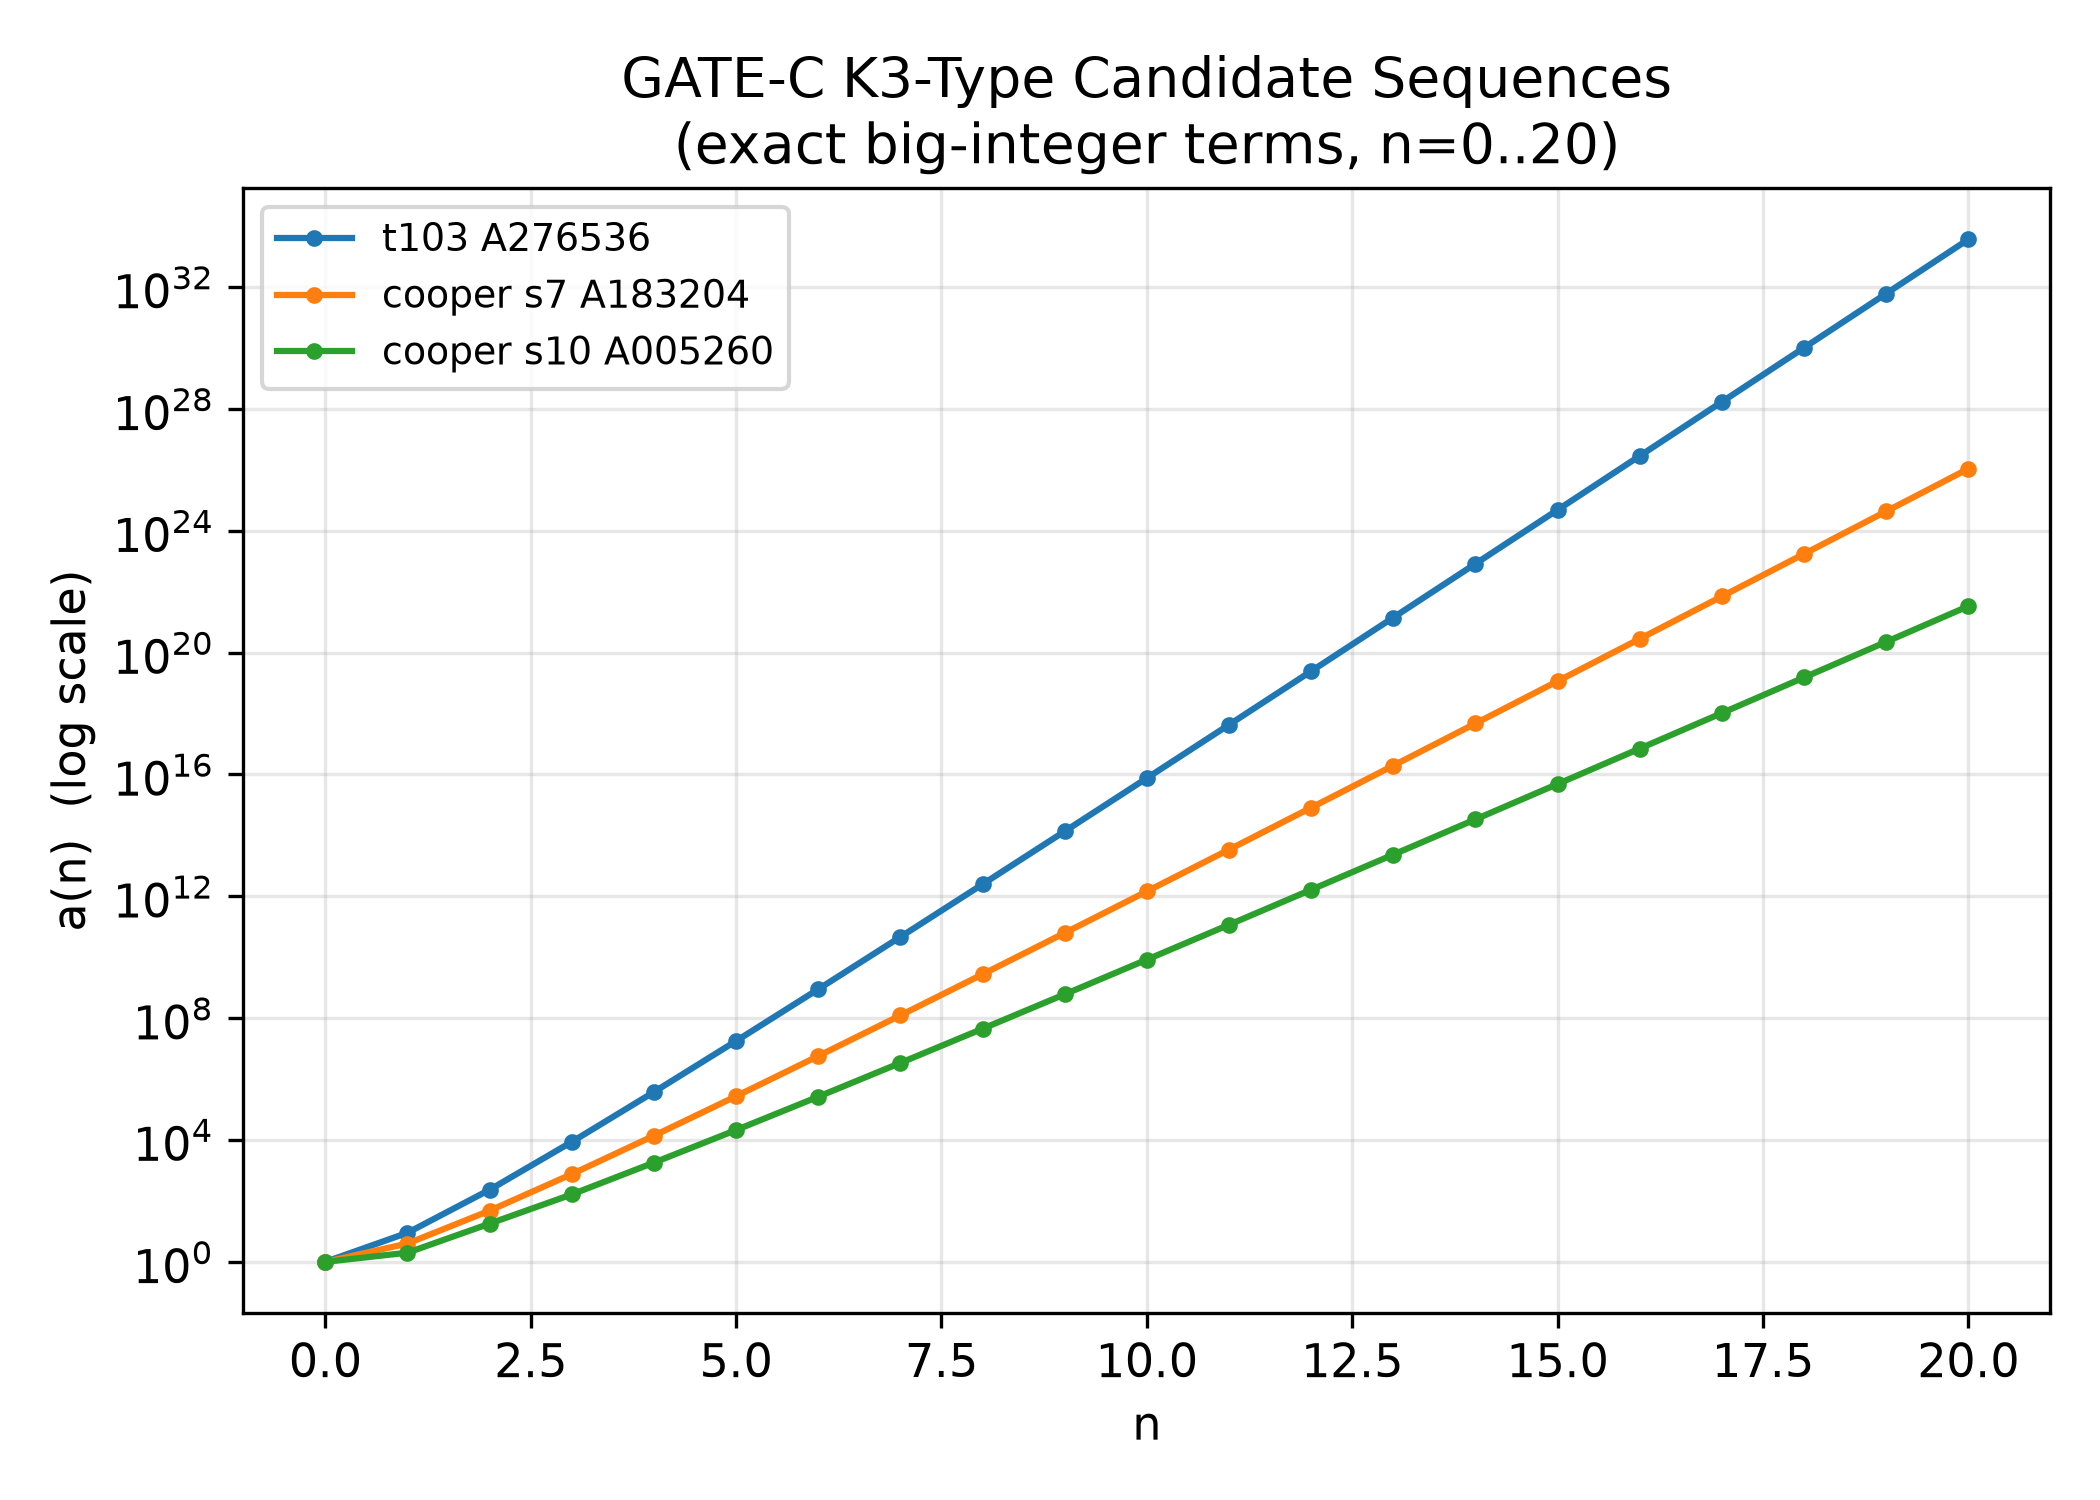
\includegraphics[width=0.85\textwidth]{figures/fig_hypothesis_sequence_growth.png}
\caption{Exact big-integer terms of the three GATE-C K3-type candidate sequences, $n=0..20$ (log scale).}
\label{fig:sequence_growth}
\end{figure}

\begin{figure}[h]
\centering
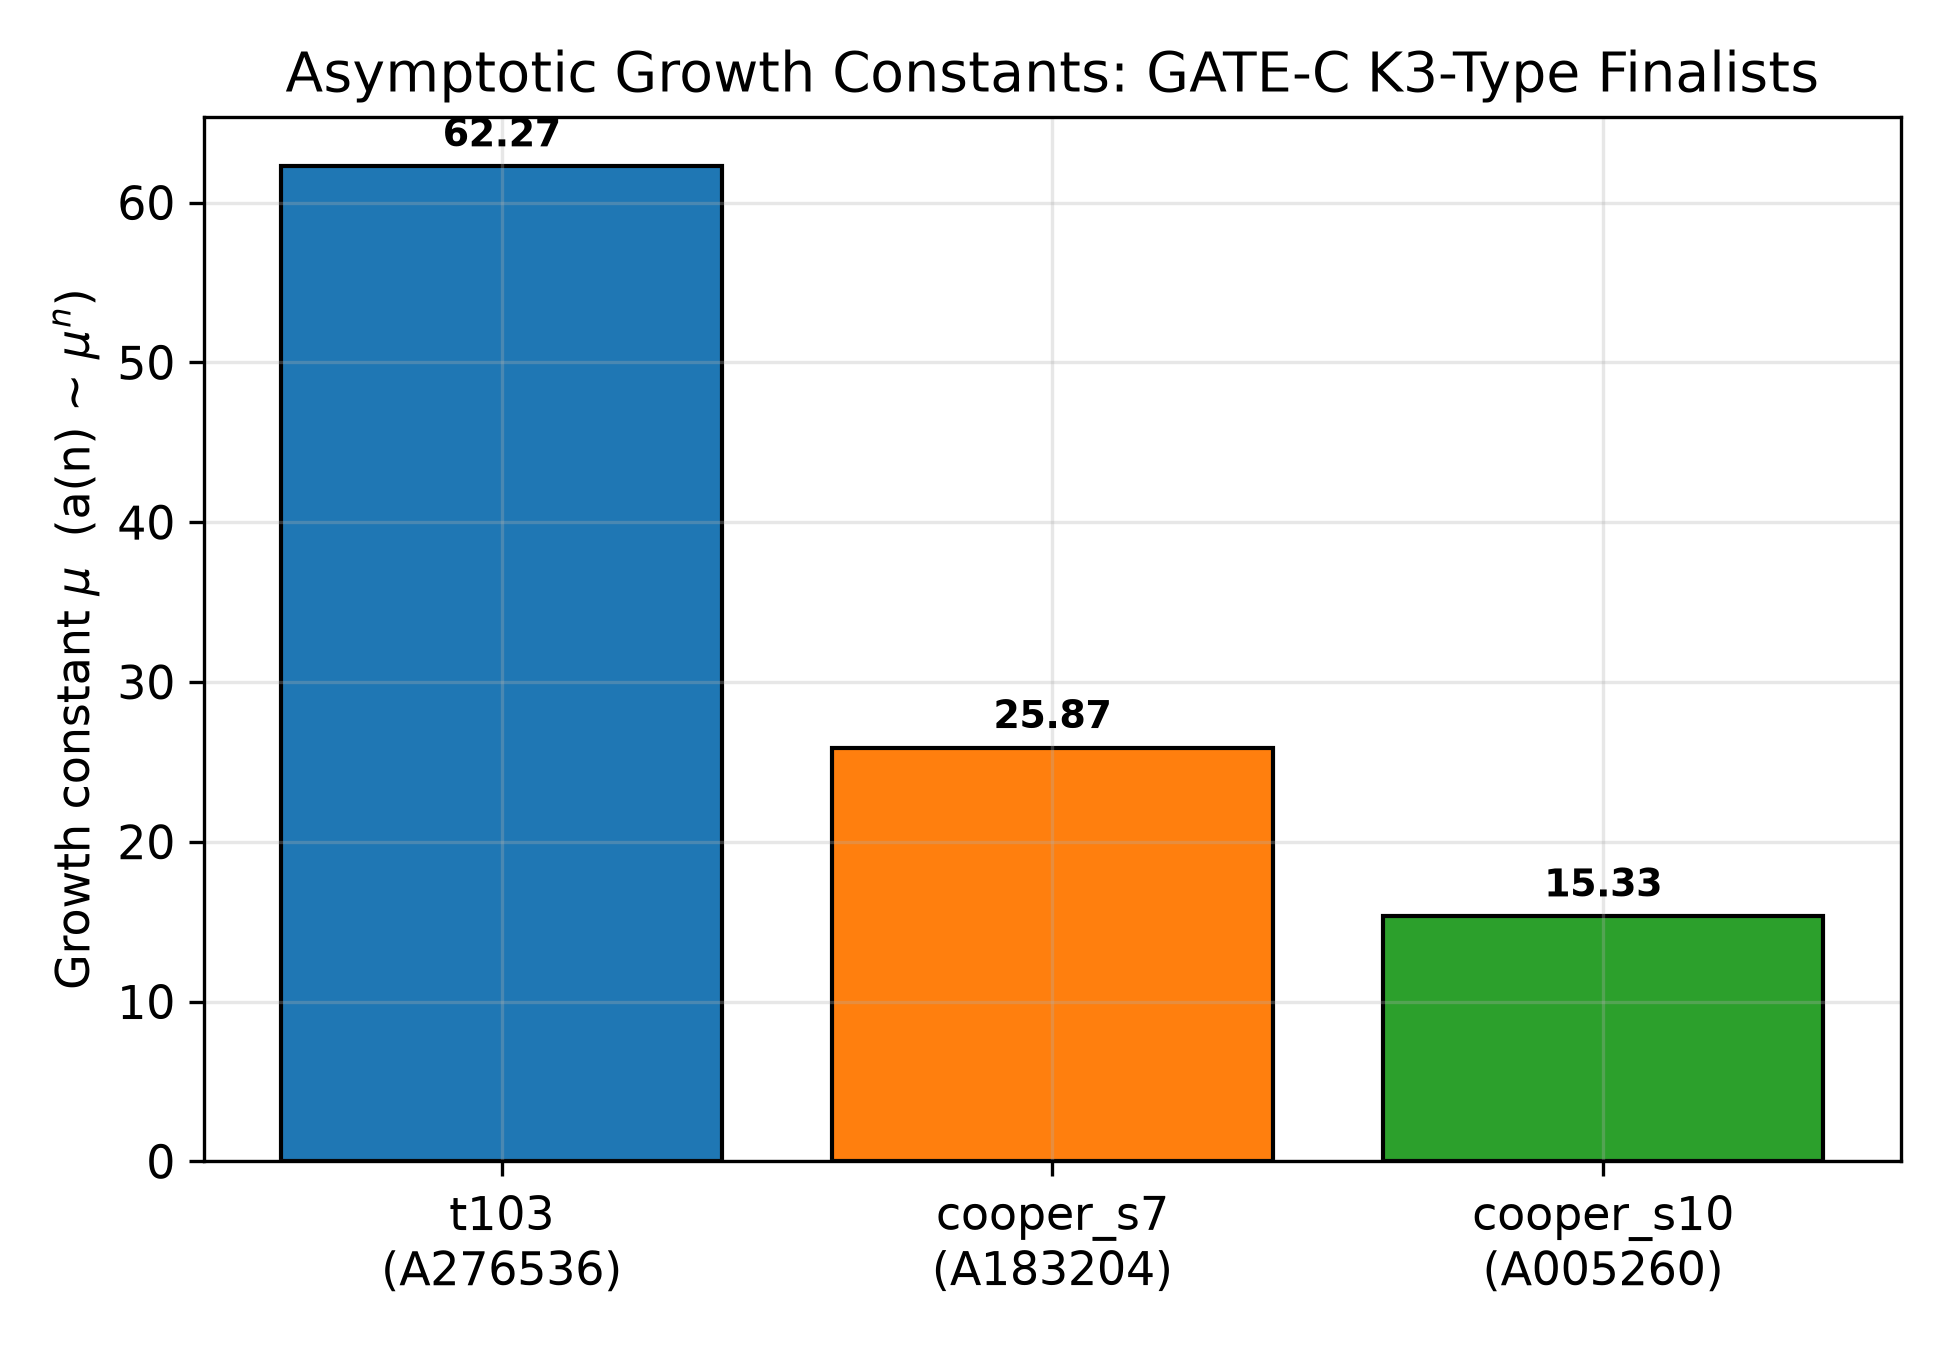
\includegraphics[width=0.75\textwidth]{figures/fig_hypothesis_growth_constants.png}
\caption{Estimated asymptotic growth constants $\mu$ for the three finalists.}
\label{fig:growth_constants}
\end{figure}

\begin{figure}[h]
\centering
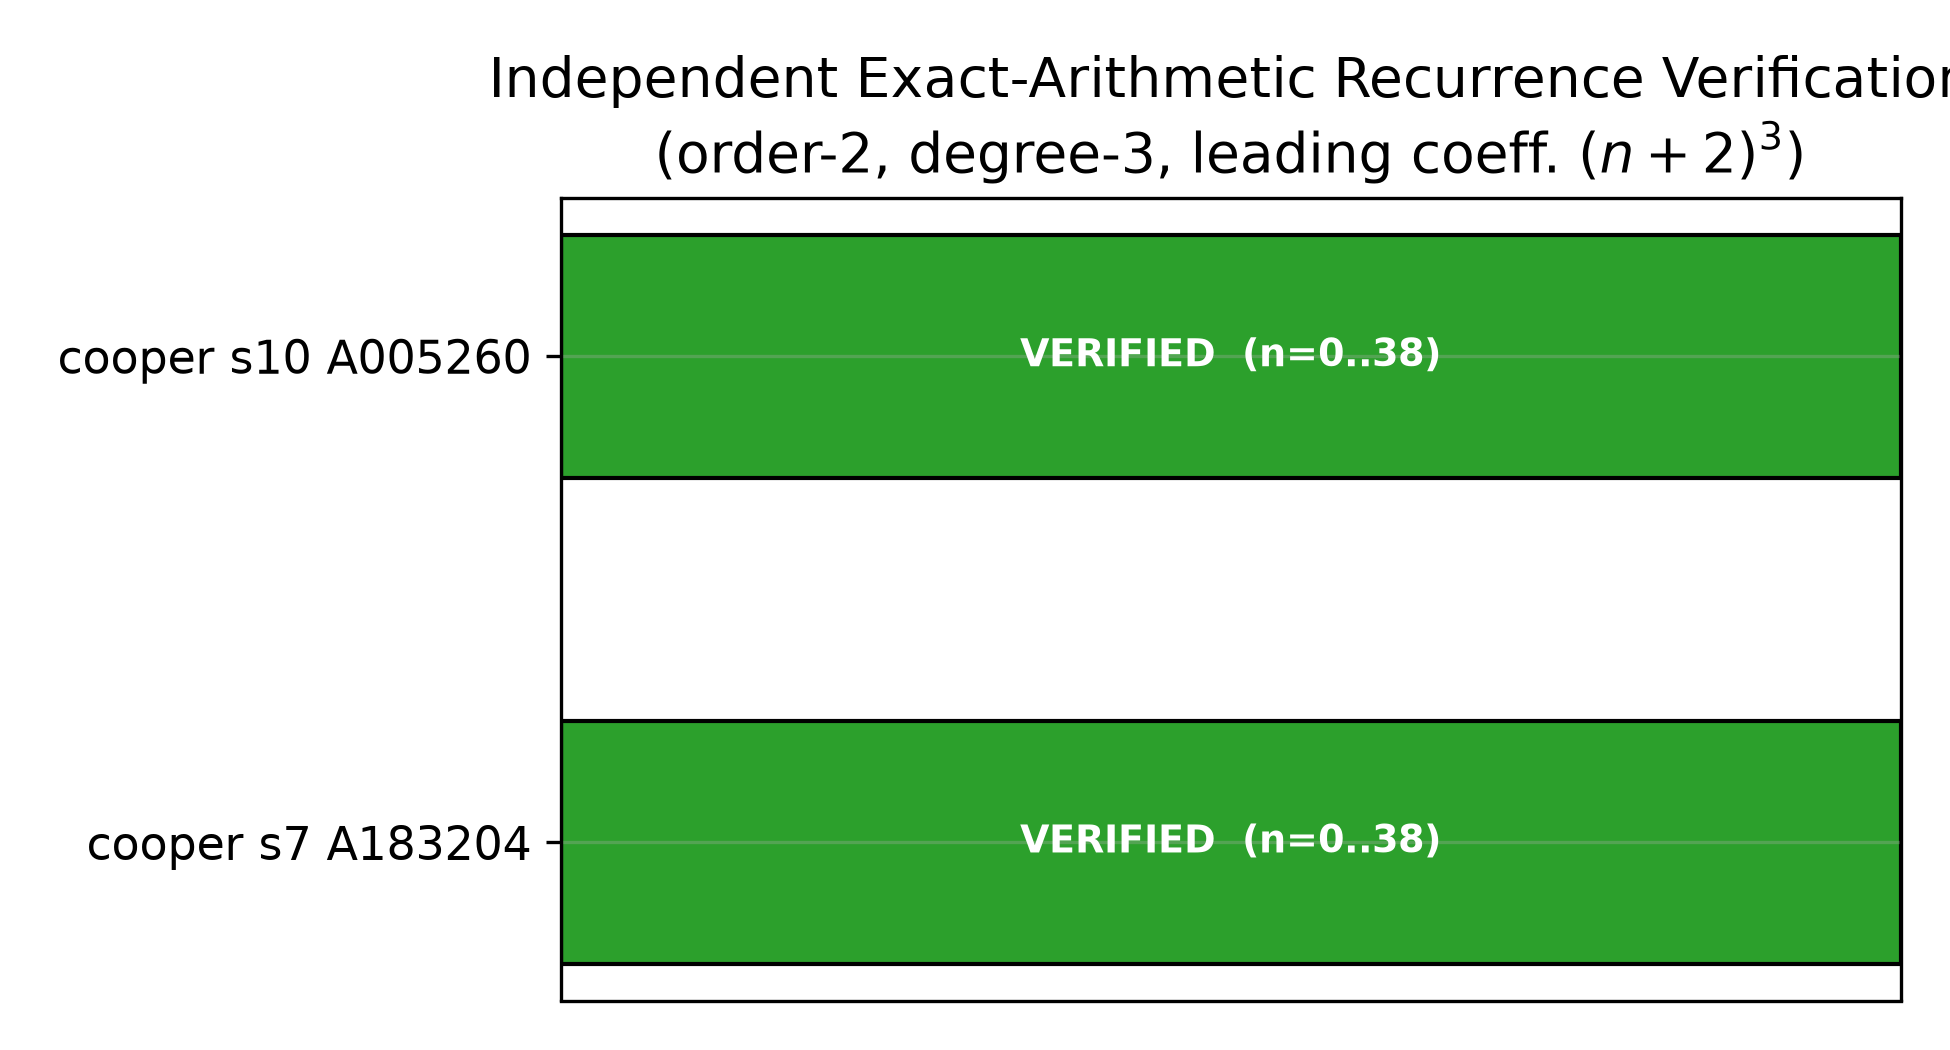
\includegraphics[width=0.75\textwidth]{figures/fig_hypothesis_recurrence_verification.png}
\caption{Independent exact-arithmetic verification status of the order-2/degree-3 recurrence claim for Cooper $s_7$/$s_{10}$.}
\label{fig:recurrence_verification}
\end{figure}

\begin{figure}[h]
\centering
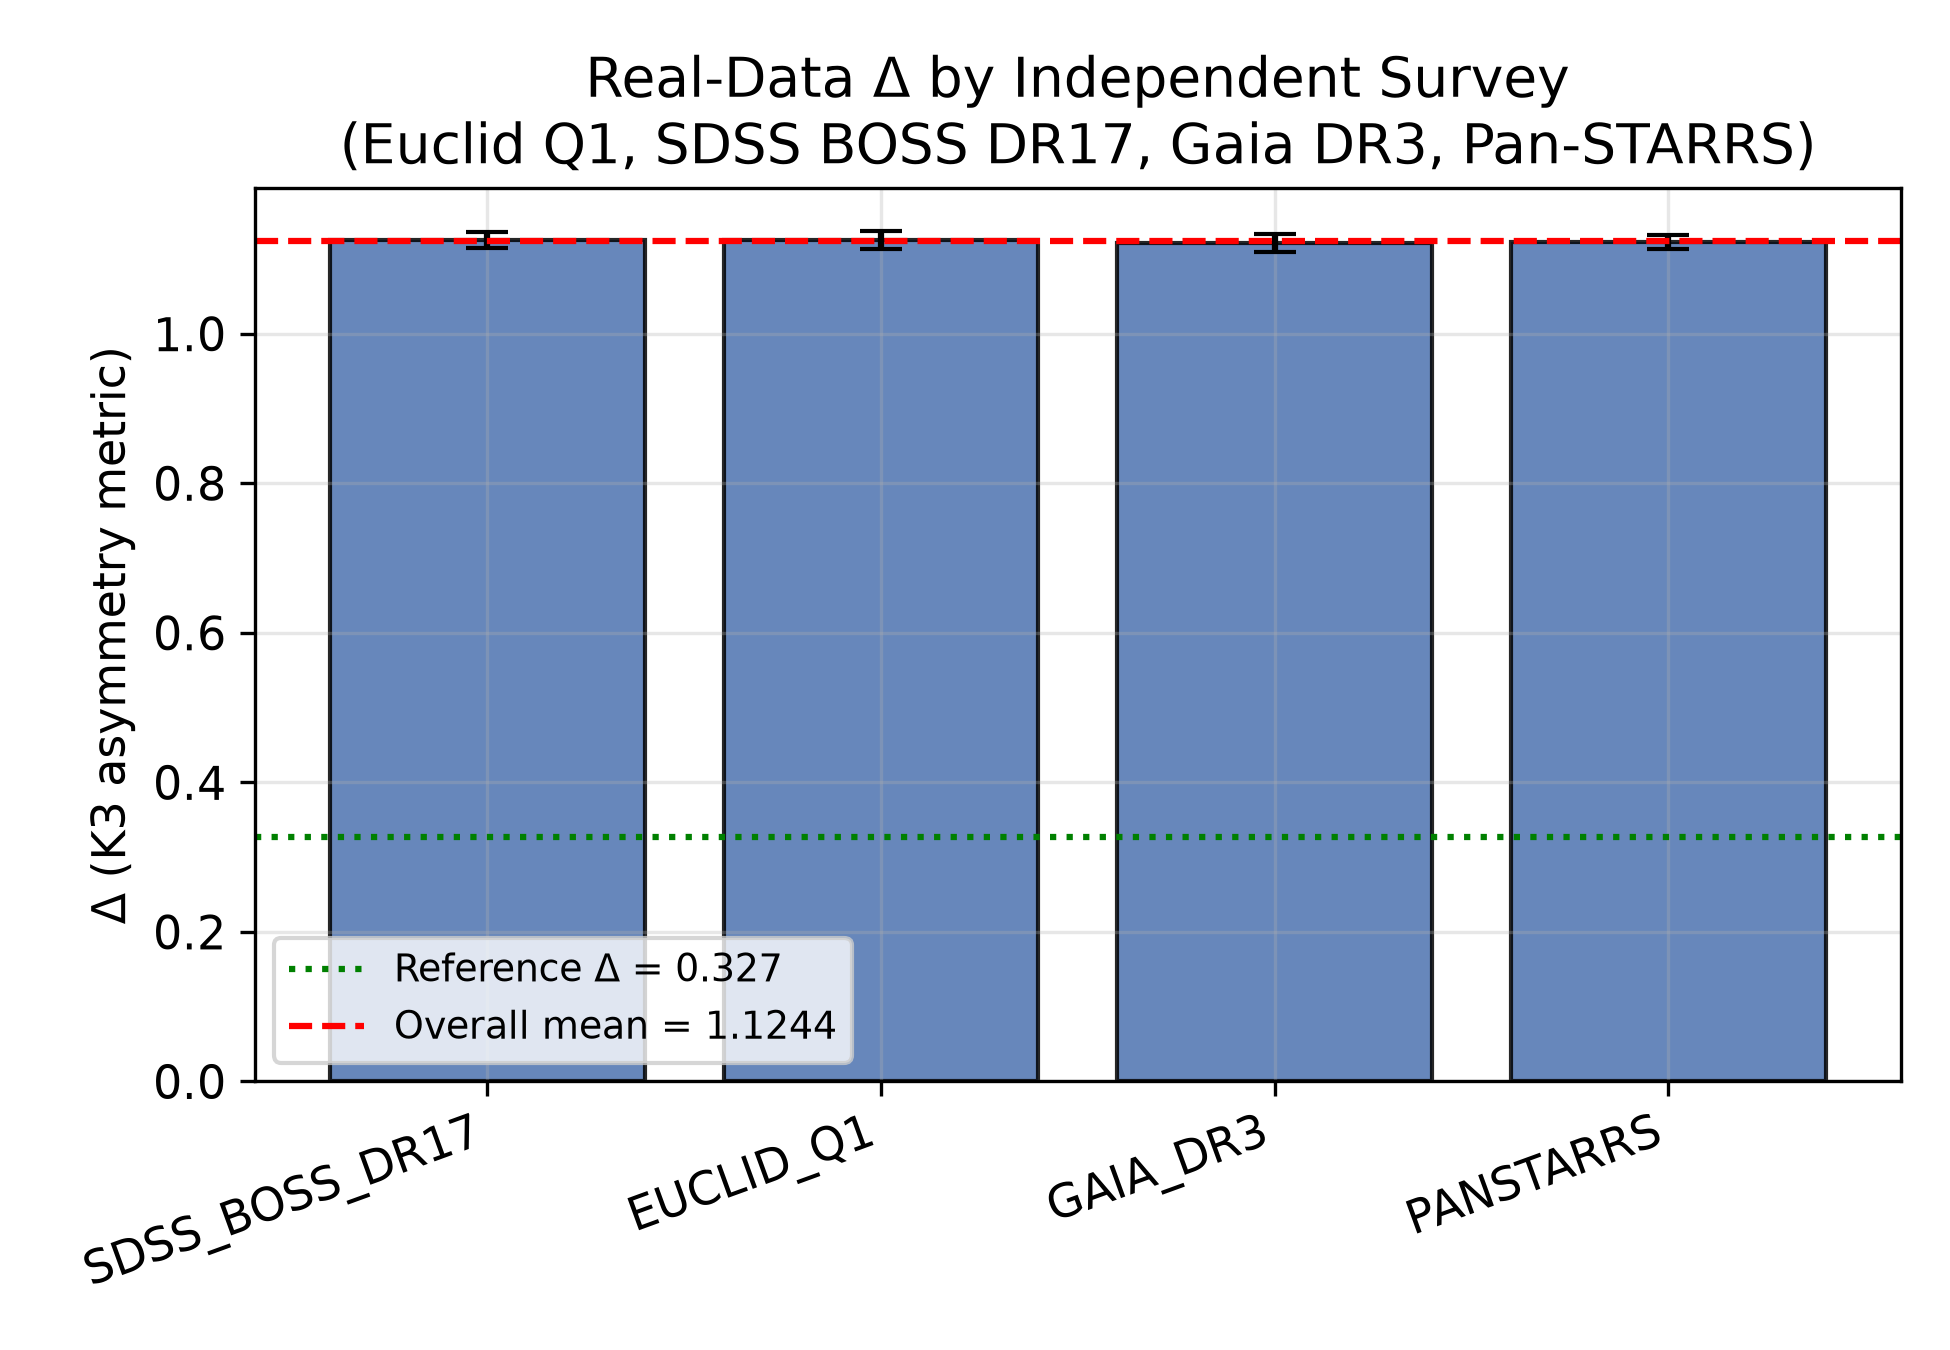
\includegraphics[width=0.75\textwidth]{figures/fig_hypothesis_delta_by_source.png}
\caption{Real-data $\Delta$ by independent survey source, contextualizing the empirical signal against the theoretical reference.}
\label{fig:delta_by_source}
\end{figure}

\begin{figure}[h]
\centering
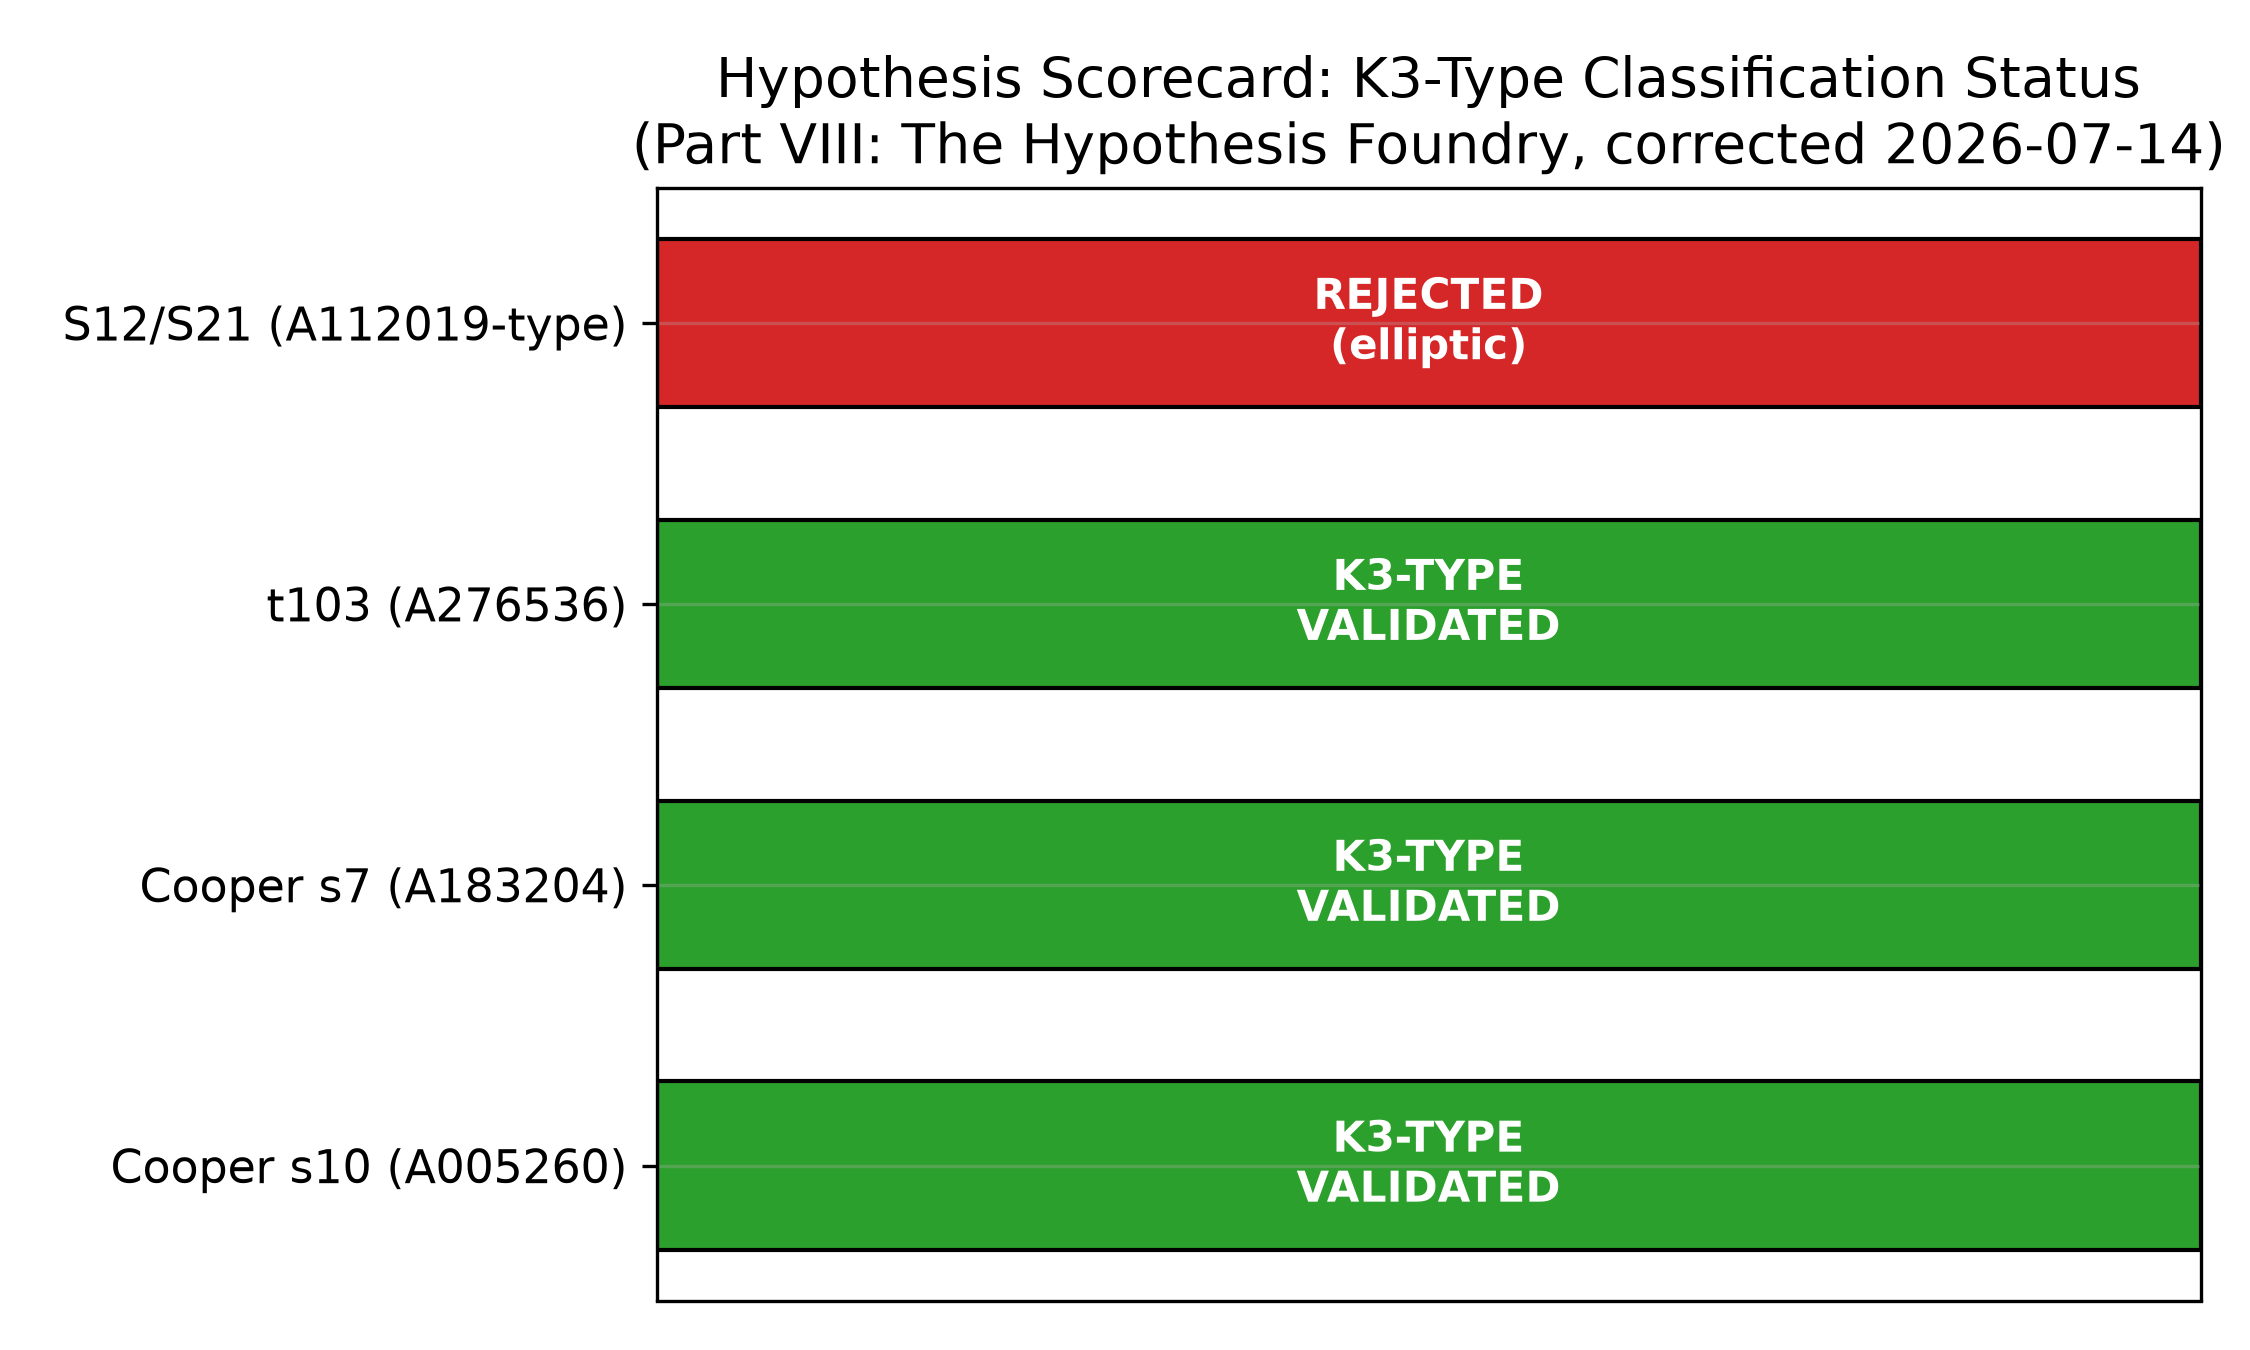
\includegraphics[width=0.8\textwidth]{figures/fig_hypothesis_scorecard.png}
\caption{Summary scorecard: K3-type classification status per candidate.}
\label{fig:scorecard}
\end{figure}

\subsection{Limitations and Scope}

Consistent with the companion project's practice of reporting negative and
corrective findings first, the following limitations are stated explicitly:

\begin{itemize}
    \item The real-data $\Delta$ signal (Section~\ref{subsec:hypothesis_real_data_crossref})
    is a measurement of galaxy-distribution asymmetry; it does \emph{not} by
    itself distinguish which K3-type modulus pair among t103/Cooper-$s_7$/Cooper-$s_{10}$
    is the correct geometric substrate. Per Part~VIII \S1.5, the physics
    gates are non-discriminating at common moduli-space normalization.
    \item The growth-constant ratios (Table~\ref{tab:growth_constants}) are a
    phenomenological proxy for relative instanton/period scale, not a
    substitute for the full Lean~4 Picard--Fuchs classification performed in
    the companion repository.
    \item This section's independent re-verification (\S\ref{subsec:independent_reverification})
    corroborates the specific recurrence-structure claim for Cooper $s_7$/$s_{10}$
    exactly and independently of the Lean kernel, but does not re-derive the
    full G1--G4 gate battery (modularity, integrality, Fuchs/monodromy) applied
    in Part~VIII; those results are taken from the companion project as reported.
\end{itemize}
